% document vide aux normes de l'école pour le mémoire

% PREAMBULE

%package obligatoire : type de document
\documentclass[a4paper,12pt,twoside]{book}

% encodage (pour XeLaTeX)
\usepackage{fontspec}

\usepackage{enumitem}
\usepackage{graphicx}
\usepackage{listings}
\usepackage{xcolor}
\usepackage{tabularx}
\usepackage{csquotes}
\usepackage{float}
\usepackage{caption}
\usepackage{subcaption}

\newcommand{\clearemptydoublepage}{\newpage{\pagestyle{empty}\cleardoublepage}}

\definecolor{codegreen}{rgb}{0,0.6,0}
\definecolor{codegray}{rgb}{0.5,0.5,0.5}
\definecolor{codepurple}{rgb}{0.58,0,0.82}
\definecolor{backcolour}{rgb}{0.95,0.95,0.92}

\lstdefinestyle{pythonStyle}{
    backgroundcolor=\color{backcolour},   
    commentstyle=\color{codegreen},
    keywordstyle=\color{magenta},
    numberstyle=\tiny\color{codegray},
    stringstyle=\color{codepurple},
    basicstyle=\ttfamily\footnotesize,
    breakatwhitespace=false,         
    breaklines=true,                 
    captionpos=b,                    
    keepspaces=true,                 
    numbers=left,                    
    numbersep=5pt,                  
    showspaces=false,                
    showstringspaces=false,
    showtabs=false,                  
    tabsize=2
}

\definecolor{codegray}{rgb}{0.5,0.5,0.5}
\lstdefinestyle{YMLStyle}{
    backgroundcolor=\color{white},
    commentstyle=\color{codegray},
    keywordstyle=\color{blue},
    numberstyle=\tiny\color{codegray},
    stringstyle=\color{red},
    basicstyle=\ttfamily\small,
    breakatwhitespace=false,
    breaklines=true,
    captionpos=b,
    keepspaces=true,
    numbers=left,
    numbersep=5pt,
    showspaces=false,
    showstringspaces=false,
    showtabs=false,
    tabsize=2
}

\lstdefinestyle{jsonStyle}{
  basicstyle=\ttfamily,
  columns=fullflexible,
  showstringspaces=false,
  commentstyle=\color{gray},
  keywordstyle=\color{blue},
  stringstyle=\color{red},
  frame=single,
  breaklines=true,
  breakatwhitespace=true,
  captionpos=b,
  numbers=left,
  numberstyle=\tiny\color{gray}
}

\lstdefinestyle{XMLStyle}{
  language=XML,
  basicstyle=\ttfamily,
  keywordstyle=\color{blue},
  stringstyle=\color{red},
  commentstyle=\color{green},
  morestring=[b]",
  morestring=[s]{>}{<},
  morecomment=[s]{<?}{?>},
  morecomment=[s][\color{red}]{<!--}{-->}
}


%si index, package pour index + makeindex avant hyperref


% le package hyperref avec des options, si en local
%\usepackage[pdfusetitle, pdfsubject ={Mémoire TNAH}, pdfkeywords={les mots-clés}]{hyperref}

%avec overleaf, utiliser :
\usepackage[xetex]{hyperref}
\hypersetup{
pdfauthor = {Samuel Scalbert},
pdftitle = {Les CMS et le low-code au service des humanités numériques : l'exemple de DiScholEd, une application TEI Publisher},
pdfsubject = {sujet},
pdfkeywords = {TEI Publisher} {DiScholEd} {XML} {Python} {JavaScript} {Exide} {CMS} {Inria} {low-code}}

%il faut mettre au moins une langue
\usepackage[english,french]{babel}

% configurer le document selon les normes de l'école
\usepackage[margin=2.5cm]{geometry} %marges
\usepackage{setspace} % espacement qui permet ensuite de définir un interligne
\onehalfspacing % interligne de 1.5
\setlength\parindent{1cm} % indentation des paragraphes à 1 cm

\usepackage{lettrine} % lettrines (pas obligatoire)


% bibliographie
\usepackage[backend=biber, sorting=nyt, style=enc,maxbibnames=10]{biblatex}
\addbibresource{main/reference.bib}
\nocite{*}

\usepackage{glossaries}
\makeglossaries


% + toutes la liste des packages nécessaires à votre document (si images, tableaux, schémas, etc.)

% on pourra aussi utiliser la commande mise dans l'exemple de correction du TP1 pour enlever les titres courant qui traînent sur les pages

\author{Prénom Nom - M2 TNAH}
\title{Titre du mémoire}

% DOCUMENT
\begin{document}
	\begin{titlepage}
		\begin{center}
			
			\bigskip
			
			\begin{large}				
				ÉCOLE NATIONALE DES CHARTES\\
				UNIVERSITÉ PARIS, SCIENCES \& LETTRES
			\end{large}
			\begin{center}\rule{2cm}{0.02cm}\end{center}
			
			\bigskip
			\bigskip
			\bigskip
			\begin{Large}
				\textbf{Samuel Scalbert}\\
			\end{Large}
		%selon le cas
			\begin{normalsize} \textit{licencié ès lettres}\\
				\textit{diplômé de master}
			\end{normalsize}
			
			\bigskip
			\bigskip
			\bigskip
			
			\begin{Huge}
				\textbf{Les CMS et le low-code au service des humanités numériques : l'exemple de DiScholEd, une application TEI Publisher}\\
			\end{Huge}
			\bigskip
			
			\bigskip
			\bigskip
			\begin{large}
			\end{large}
			\vfill
			
			\begin{large}
				Mémoire 
				pour le diplôme de master \\
				\og{} Technologies numériques appliquées à l'histoire \fg{} \\
				\bigskip
				2023
			\end{large}
			
		\end{center}
	\end{titlepage}
	
	\thispagestyle{empty}	
	\clearemptydoublepage
	
	\frontmatter
	\chapter{Résumé}
	\medskip
   Le projet DiScholEd est dédié à la gestion de sept corpus datant du XIX\up{e} et du XX\up{e} siècle, lesquels sont rendus accessibles via une plateforme web. Ces corpus sont principalement constitués de documents personnels, souvent qualifiés d'ego-documents. En septembre 2023, notre application compte une collection de 714 documents. Dans le cadre de cette mise en ligne, notre choix s'est orienté vers l'utilisation d'un CMS (Système de Gestion de Contenu), à savoir TEI Publisher. Les CMS ont acquis une importance indéniable dans le domaine du développement web. Le but de ce mémoire est d'analyser dans quelle mesure TEI Publisher s'adapte efficacement au projet DiScholEd.\\
	
	\textbf{Mots-clés~:}TEI Publisher~; Publisher~; XML TEI~; Python~; JavaScript~; low-code~; CMS~; Inria
	
	\textbf{Informations bibliographiques~:} Samuel Scalbert, \textit{Les CMS et le low-code au service des humanités numériques : l'exemple de DiScholEd, une application TEI Publisher}, mémoire de master \og{}Technologies numériques appliquées à l'histoire\fg{}, dir. [Floriane Chiffoleau et Jean-Damien Généro], École nationale des chartes, 2023.
	
	\clearemptydoublepage
	
	\chapter{Remerciements}
	
	\lettrine{J}e tiens tout d'abord à exprimer ma gratitude envers toutes les personnes qui m'ont soutenu au cours de ma deuxième année de Master.

Je souhaite particulièrement remercier mes tuteurs, Jean-Damien Généro et Floriane Chiffoleau, qui m'ont accompagné avec bienveillance et qui ont constamment partagé d'excellents conseils. J'adresse également mes remerciements à tous les membres de l'équipe ALMAnaCH d'Inria pour leurs précieux conseils. Je souhaite exprimer ma gratitude envers Sarah, qui a été une camarade exceptionnelle pendant la durée de notre stage.

    \chapter*{Liste des sigles et abréviations}
\addcontentsline{toc}{chapter}{Liste des sigles et abréviations}

\begin{center}
\textit{Institutions}
\end{center} 

\begin{itemize}
    \item ALMAnaCH : \textit{Automatic Language Modelling and Analysis \& Computational Humanities} (Inria Paris)
    \item EHESS : École des Hautes Études en Sciences Sociales
    \item Inria : Institut national de recherche en informatique et en automatique
    \item MESRI : Ministère français de l’Enseignement supérieur, de la Recherche et de l’Innovation
\end{itemize}

\bigbreak

\begin{center}---

\bigbreak

\textit{Programmes de recherche}
\end{center} 

\begin{itemize}
    \item DAHN : Dispositif de soutien à l’Archivistique et aux Humanités Numériques (\textit{Digital edition of historical manuscripts})
\end{itemize}

\begin{center}---

\bigbreak

\textit{Informatique et nouvelles technologies}
\end{center} 

\bigbreak

\begin{itemize}
    \item API : \textit{Application Programming Interface}
    \item CSV : \textit{Comma-separated values}
    \item HTML : \textit{Hypertext Markup Language}
    \item ODD: \textit{One Document Does it all}
    \item PDF : \textit{Portable Document Format}
    \item TEI : \textit{Text Encoding Initiative}
    \item XML : \textit{eXtensible Markup Language}
    \item Xquery : \textit{XML Query}
    \item CMS : \textit{Content Management System}
    \item ODD : \textit{One Document Does it all}
    \item UX : \textit{User Experience}
    \item URL : \textit{Uniform Resource Locator}
    \item SEO : \textit{Search Engine Optimization}
\end{itemize}

\clearpage
\thispagestyle{empty}
	\clearemptydoublepage
 
	\chapter*{Introduction}
\addcontentsline{toc}{chapter}{Introduction}

La transformation numérique des données extraites de collections d'archives, ainsi que leur diffusion au public sous forme de documents numériques dans divers formats et/ou sous forme d'éditions en ligne, représentent un défi majeur dans le domaine de la recherche et de la préservation du patrimoine culturel. Le projet DAHN, fruit d'une collaboration technologique et scientifique entre l'Inria, l'Université du Mans et l'École des hautes études en sciences sociales (EHESS), financé par le ministère français de l'Enseignement supérieur, de la Recherche et de l'Innovation, s'est engagé à relever ce défi.

DiScholEd (\textit{Digital Scholarly Editions}) a alors été créée pour la mise en ligne des documents numériques. Le projet, en septembre 2023, compte sept corpus. Pour la publication des résultats de la \textit{pipeline} du projet, le choix a été fait d'utiliser un CMS (Content Management System) spécialisé dans les éditions numériques : TEI Publisher.

TEI Publisher est un CMS qui vise à permettre à des chercheurs n'ayant pas de compétences en informatique de publier leurs éditions numériques en ligne. DiScholEd ne dispose pas de développeur attitré au projet, il était donc nécessaire d'utiliser un CMS qui utilise le \textit{low-code} tel que TEI Publisher.

Le \textit{low-code} pour les CMS est une approche de développement web qui repose sur l'utilisation de plateformes ou d'outils générant automatiquement une partie du code nécessaire pour créer des sites web ou des applications web. Contrairement au \textit{no-code} (une approche qui empêche de coder directement l'application), le \textit{low-code} permet généralement un niveau de personnalisation et de contrôle plus élevé en permettant aux utilisateurs de modifier le code généré ou d'ajouter des éléments personnalisés si nécessaire. Cela rend le \textit{low-code} adapté aux projets nécessitant une plus grande flexibilité tout en réduisant la quantité de code à écrire manuellement, ce qui accélère le processus de développement.

Dans son article sur les éditions scientifiques numériques, Elena Pierazzo soulève des questions cruciales sur l'utilisation des outils numériques et de la recherche textuelle\footcite{pierazzo:hal-02117714}. Elle se demande si les chercheurs doivent être en mesure d'utiliser ces outils eux-mêmes, si une assistance est nécessaire pour la configuration des éditions et qui devrait fournir cette assistance ?

Notre mémoire vise à réaliser une étude de cas autour de DiScholEd et de TEI Publisher. L'objectif est d'analyser si TEI Publisher est adapté à notre projet et si le \textit{low-code} nous permet de créer notre application sans l'aide d'un développeur tout en produisant une application originale.

Ce mémoire est structuré en trois parties. Dans la première partie, nous présenterons le contexte du projet DiScholEd et de ses corpus, ainsi que les caractéristiques essentielles des CMS, en mettant particulièrement l'accent sur TEI Publisher. Nous aborderons également la gestion des erreurs dans TEI Publisher.

La deuxième partie se penchera sur les avantages et les inconvénients de TEI Publisher, basés sur les travaux réalisés pendant le stage. Nous analyserons trois aspects cruciaux qui orientent le choix d'un CMS lors du développement d'une application web : la gestion des erreurs, la personnalisation des fonctionnalités et la possibilité de créer un design propre à notre application.

Enfin, la troisième partie explorera les perspectives d'amélioration de TEI Publisher et de l'application DiScholEd. Nous évaluerons l'adéquation de TEI Publisher pour différents types d'utilisateurs en mettant en évidence les défis liés à l'équilibre entre facilité d'utilisation et personnalisation pour les chercheurs. Nous proposerons ensuite des améliorations potentielles pour TEI Publisher et discuterons des évolutions futures possibles pour l'application DiScholEd.
	\clearemptydoublepage
    % bibliographie ici
    \printbibliography[heading=bibintoc,keyword=main,title={Bibliographie générale}]
    \printbibliography[heading=bibintoc,keyword=site,title={Sites Internet}]
	\clearemptydoublepage
 
	\mainmatter
	
	% là, le corps du mémoire, généralement TROIS parties
	
	% possibilité d'avoir un document main.tex peu rempli, et chaque partie appelée par \input{} par exemple
    
    \clearemptydoublepage
    \part{DiScholEd, une application développée avec le CMS TEI Publisher}

\chapter{Les corpus de DiScholEd }

Originellement, l'application présentait deux collections: les lettres et textes des intellectuels berlinois et la correspondance de Paul d’Estournelles de Constant. DiScholed possède en septembre 2023 sept corpus que l'on peut regrouper dans deux catégories différentes : les corpus du XIX\up{e} siècle et les corpus du XX\up{e} siècle. Les corpus sont en français, tchèque, allemand, anglais, hongrois, yiddish, latin, grec et italien.

\section{Les corpus XIX\up{e} siècle}

\subsection{Lettres et textes : Le Berlin intellectuel des années 1800}

Ce corpus est composé de lettres et de textes d’une dizaine d’intellectuels berlinois du début du XIX\up{e} siècle, parmi lesquels August Boeckh (1785-1867), Adelbert von Chamisso (1781-1838) et Ludwig Tieck (1773-1853). Ces auteurs ont participé à la naissance du romantisme allemand, un mouvement littéraire qui valorise l’imagination, le sentiment et la nature. Ils ont également fréquenté les cercles intellectuels de Berlin, où ils ont échangé leurs idées et leurs œuvres. Ce corpus illustre la diversité et la richesse de la culture allemande à cette époque. Le corpus comprend des documents personnels, mais aussi des œuvres de fiction (nouvelles, pièces de théâtre) et des travaux scientifiques (thèse). Le corpus a déjà fait l’objet d’une édition et d’une publication\footcite{DiScholEdBerlinintellectualsCorrespondences}, mais il nécessitait une mise à jour et une migration vers une plateforme de publication plus pérenne.

\subsection{Journal des guerres napoléoniennes}

Le fonds \og{}Nachlass Böttiger, Carl August (1760-1835) Saxonica und Sammlungen zur Zeitgeschichte\fg{}\footcite{bottigerNachlassBottigerCarl00} est un fonds d’archives conservé à la Bibliothèque d’État et Universitaire de Saxe (SLUB) à Dresde. Il contient le legs de Carl August Böttiger (1760-1835), un écrivain, journaliste et archéologue allemand, qui fut proche des représentants de la \textit{Weimarer Klassik}, le mouvement littéraire et culturel allemand du XVIIIe siècle. Le fonds comprend 297 volumes et capsules, dont une grande partie est constituée d'échanges de lettres avec Böttiger, ainsi que des documents sur l’histoire de la Saxe et de l’Allemagne.
    
Le corpus sur DiScholEd contient le manuscrit intitulé \og{}\textit{Journal des événements de Leipzig du 10 octobre [1813]}\fg{}. Il est rédigé par Friedrich Rochlitz (1769-1842) un écrivain, librettiste, biographe et critique musical saxon. Il s'agit d'un témoignage historique sur la bataille de Leipzig, qui opposa les armées de Napoléon à celles de la coalition formée par la Russie, la Prusse, l’Autriche et la Suède. Cette bataille se solda par une défaite française et marqua le début du déclin de l’Empire napoléonien. Le manuscrit relate les événements du 10 octobre 1813, jour où Napoléon lança une offensive contre les positions ennemies au sud de Leipzig.
    
\subsection{Correspondance de Constance de Salm (1767-1845)}

Constance de Salm (1767-1845) est une écrivaine française éminente de son époque. Originaire de Nantes, sous le nom de Constance Marie de Théis, elle publie ses premiers essais à 18 ans. Sa notoriété s'affirme en 1794 avec le livret du drame musical \og{}\textit{Sapho}\fg{}. Elle laisse derrière elle de nombreux poèmes et panégyriques acclamés, ainsi qu'un roman intitulé \og{}\textit{Vingt-quatre heures de la vie d'une femme sensible}\fg{}. Ses œuvres abordent des enjeux socio-politiques contemporains, notamment l'éducation des femmes et leur place dans la société. Constance de Salm est la première femme admise au sein du cercle de l'Athénée des arts à Paris, une association regroupant artistes et érudits. À travers son salon parisien, elle réunit un cercle prestigieux d'amis, parmi lesquels des écrivains, des chercheurs et des artistes éminents de son temps. Cette correspondance étendue est menée de front avec ces personnalités.

Le corpus de lettres de Constance de Salm est composé d'environ 11 000 lettres et documents conservés dans deux archives distinctes (le fond \og{}Salm\fg{} de la Société des Amis du Vieux Toulon et de sa Région et d'autre part de la collection \og{}Constance de Salm\fg{} des archives du \og{}Schloss Dyck\fg{} de la \og{}\textit{Vereinigte Adelsarchive im Rheinland e.V.}\fg{}). Ces documents sont divisés en deux parties principales : les transcriptions que Constance de Salm a faites de son vivant pour préparer l'édition de sa correspondance et les lettres originales. Datant principalement des années 1798 à 1844, ce corpus regroupe environ 350 auteurs et destinataires variés. Le contenu de ces lettres offre une perspective unique sur la vie littéraire et scientifique à Paris pendant cette période. Ces documents éclairent les enjeux et les conditions de l'écriture féminine, tout en illustrant les mécanismes des réseaux et des échanges culturels entre le Rhineland et la France au XIXe\up{e} siècle.

\subsection{August Boeckh - Catalogue de ses manuscrits}

August Boeckh, philologue classique (1785-1867) est connu pour l'histoire des sciences et la politique scientifique. Au sein de l'Académie des sciences de Prusse, Boeckh a promu la recherche scientifique en lançant des projets d'envergure, notamment le projet du \og{}\textit{Corpus Inscriptionum Graecarum}\fg{}. À partir de 1811, il a entamé sa carrière d'enseignant à l'université de Berlin, où il a également contribué à façonner la structure de l'institution. Il occupe alors les postes suivants: doyen de la faculté des arts et des sciences humaines, recteur de l'université, et fondateur du séminaire philologique en 1812.

Le projet Boeckh Nachlassprojekt a été créé pour cataloguer les manuscrits rédigés de la main d'August Boeckh lui-même ou dans lesquels il a laissé une marque significative. Cette collection comprend une grande quantité de documents issus de ses nombreuses activités en tant que doyen, président de diverses commissions et directeur du séminaire philologique à l'université de Berlin entre 1811 et sa disparition en 1867. \footcite{DiScholEdBerlinintellectualsCorrespondences}

\section{Les corpus XX\up{e} siècle}

\subsection{Correspondance de d'Estournelles de Constant}

Ce corpus regroupe les échanges de Paul d’Estournelles de Constant (1852-1924), diplomate et homme politique français, avec Nicholas Murray Butler, universitaire et homme politique américain. Ces deux hommes, lauréats du prix Nobel de la paix (en 1909 pour Paul d’Estournelles de Constant et 1931 pour Nicholas Murray Butler), ont entretenu une relation épistolaire régulière entre 1914 et 1924. Ils ont partagé leurs expériences, leurs opinions et leurs sentiments sur le conflit, tout en défendant leur idéal pacifiste et leur projet d’organisation mondiale. Ce corpus présente un intérêt historique et littéraire, car il s’agit de documents personnels qui témoignent à la fois de la vie quotidienne et des enjeux politiques de l’époque. Le corpus est également riche, puisqu’il comprend environ 1500 lettres, de longueur variable, rédigées à la machine à écrire.

\subsection{Ma Guerre 1914-1918}

Charles Bruneau (1883-1969) est un linguiste français, spécialiste de la langue française et de la littérature médiévale. Pendant la Première Guerre mondiale, il est mobilisé comme soldat et participe aux combats sur le front occidental. Il écrit plus de 600 lettres à sa femme et à sa famille, ainsi qu’un journal personnel, où il relate son expérience de la guerre, ses souffrances, ses espoirs et ses réflexions. De ces écrits, il tire un ouvrage intitulé \textit{Ma guerre 1914-1918}, composé d’extraits classés, datés et situés par l’auteur, qui témoignent de sa vision de la guerre et de son évolution personnelle. Ce manuscrit, resté inédit jusqu’en 2018, a été publié par les éditions Terres Ardennaises, avec la collaboration de Nicolas Beaupré, Michel Tamine (Institut Charles-Bruneau) et Jacques Lambert (Terres Ardennaises)\footcite{MaGuerre19141918}. Il constitue un document historique et littéraire de grande valeur, qui révèle le regard d’un intellectuel sur le conflit mondial et sur la langue française. Notre corpus possède aussi une annexe qui est le journal de son oncle Raymond Bruneau, demeuré à Givet durant la guerre, au chevet de son père.

\subsection{Premiers témoignages sur l'Holocauste}

Le corpus “Premiers témoignages de l’Holocauste” est un projet qui vise à rassembler, analyser et diffuser des témoignages écrits et oraux de survivants de l’Holocauste recueillis peu après la fin de la Seconde Guerre mondiale. Il s’agit d’une collaboration entre plusieurs institutions européennes, dont l’Institut d’histoire contemporaine de Munich, le Mémorial de la Shoah de Paris et le Wiener Holocaust Library de Londres. Le corpus comprend des documents en plusieurs langues, notamment l’allemand, le français, l’anglais et le yiddish. Il offre un accès à des sources historiques uniques et précieuses pour comprendre les expériences et les réactions des victimes du génocide nazi. \\

DiScholed dispose de sept corpus multilingues, tous encodés en XML conformément aux normes de la TEI (Text Encoding Initiative). Afin de les rendre accessibles en ligne, il a été décidé d'opter pour un système de gestion de contenu (CMS).

\chapter{Les CMS et TEI Publisher}

Les CMS (\textit{Content Management System}) comme TEI Publisher sont des programmes informatiques qui permettent de créer un site ou une application. Ils présentent de nombreux avantages qui facilitent considérablement le déploiement d'application. TEI Publisher est un CMS spécialement dédié aux éditions numériques. 

\section{Présentation des CMS}

Les CMS les plus connus\footcite{MeilleurCMS2023} sont \href{https://fr.wordpress.org/}{WordPress\footcite{WordPress}} ou encore \href{https://fr.wix.com/}{Wix\footcite{Wix}}. Les CMS sont aujourd'hui des références pour la création et le déploiement rapide de sites, tant pour des particuliers que pour des entreprises. 
Cette explosion\footcite{CMSOpenSource} de la popularité des CMS s'explique par le fait qu'utiliser un CMS présente de nombreux avantages. Grâce à cet outil, il est possible de considérablement réduire le temps nécessaire au développement d'un site.

Le CMS offre aussi la possibilité de développer des applications Web. En mettant à disposition une variété de \textit{plugins}, le système de gestion de contenu facilite la création d'un site sans que l'éditeur ait à se soucier du codage.

Un autre atout du CMS est son intégration native d'un créateur de page, ou \textit{page builder}, qui permet de créer, de gérer et de modifier facilement le contenu du site en utilisant des blocs dynamiques réutilisables.

La sécurité est également un point fort des CMS, car ils proposent des fonctionnalités avancées pour protéger le contenu et la base de données du site contre les tentatives d'intrusion. L'auteur du site peut aussi gérer les accès et les autorisations à l'aide des systèmes de gestion des rôle et des droits des comptes utilisateurs directement intégrés avec le CMS.

Le référencement SEO (Search Engine Optimization)  est l'ensemble des pratiques visant à optimiser la visibilité d'un site Web dans les résultats organiques des moteurs de recherche. Les CMS sont aussi optimisés pour améliorer la visibilité avec le SEO. 

Enfin, un CMS offre de meilleures possibilités de gestion et de relation utilisateur. Des fonctionnalités telles que les formulaires de contact et le chat en direct sont intégrées pour répondre aux demandes urgentes des utilisateurs.

Les chercheurs en SHS (Sciences Humaines et Sociales) ont des besoins divers en matière de gestion de contenu, que ce soit pour publier des articles, des documents de recherche, ou pour créer des plateformes collaboratives. Les CMS offrent des solutions pour toutes ces tâches.\\

Les multiples avantages qu'offre un système de gestion de contenu (CMS) sont la principale raison du choix d'opter pour cette solution. DiScholed a spécifiquement choisi TEI Publisher, un CMS spécialement conçu pour les éditions numériques, en raison de ses caractéristiques particulières.

\section{TEI Publisher}

TEI Publisher est toujours en développement et reçoit des mises à jour majeures deux fois par an, apportant de nouvelles fonctionnalités et corrigeant les \textit{bugs}. L'objectif est de permettre aux chercheurs et aux éditeurs de publier leurs documents rapidement, facilement et avec des compétences minimales en programmation. 

TEI Publisher est une application open source pour eXist-db (une plateforme de développement pour les applications basées sur XML). Elle est compatible avec les documents TEI (Text Encoding Initiative) tout en offrant la possibilité d'être adaptée à n'importe quel autre schéma\footcite{AtomicWiki}. Elle permet de publier une édition numérique sans écrire de code. En utilisant le modèle de traitement TEI, la personnalisation de l’apparence du texte se fait entièrement en XML. TEI Publisher produit des applications qui intègrent déjà des fonctionnalités telles que la navigation page par page, la fonction de recherche, et la possibilité d'exporter vers différents formats.\footcite{TEIPublisherDocumentation}

TEI Publisher est un projet collaboratif basé sur les idées et les contributions du monde entier. Il a été initialement inspiré par la vision derrière le modèle de traitement TEI \og{}travail du défunt Sebastian Rahtz et d’autres membres du projet TEI Simple de 2015\fg{}\footcite{TEIPublisher} et continue d’évoluer. Il est sous licence GPLv3 et fonctionne grâce à Exist-db.

Exist-db simplifie grandement la gestion du \textit{back-end}, qui fait référence à la partie invisible d'une application informatique, celle qui gère les données, les processus et la logique sous-jacente. Contrairement à l'interface utilisateur visible du logiciel (appelée le \textit{front-end}), le back-end travaille en coulisses pour garantir le bon fonctionnement de l'application. Pour gérer le \textit{back-end} plusieurs logiciels sont fournis avec exist-db:

\begin{itemize}[label=\textbullet]
    \item eXide - XQuery IDE : eXide est un environnement de développement intégré (IDE) pour XQuery qui permet de développer et de déboguer des applications XQuery pour eXist-db.
    \item eXist-db Demo Apps : Les applications de démonstration d’eXist-db montrent comment utiliser les fonctionnalités d’eXist-db pour créer des applications Web.
    \item eXist-db Documentation : La documentation d’eXist-db fournit des informations détaillées sur l’utilisation et la configuration d’eXist-db, ainsi que sur les fonctionnalités et les API (\textit{Application Programming Interface} ou \og{}Interface de Programmation Applicative\fg{} est un ensemble de règles et de protocoles permettant à l'application de communiquer et d'échanger des données avec le serveur) disponibles.
    \item Monex : Monex est un outil de surveillance et de gestion de performances pour eXist-db qui permet de surveiller les performances du serveur et de diagnostiquer les problèmes.
    \item XQuery Function Documentation : La documentation des fonctions XQuery fournit une référence complète des fonctions XQuery disponibles dans eXist-db.
\end{itemize}

La documentation officielle de TEI Publisher se décrit comme: \og{}un outil qui permet aux chercheurs et aux éditeurs de publier leurs travaux sans devenir des programmeurs, tout en ne les contraignant pas à un cadre universel. Les développeurs expérimentés en bénéficieront également\fg{}\footcite{TEIPublisher}. Pour aider les non-programmeurs, TEI Publisher a fait d'intégrer le \textit{low-code} avec la mise en place d'une interface graphique pour modifier l'ODD et des fonctionnalitées déjà fonctionnelles dans les applications.
C'est pourquoi TEI Publisher semble être un choix idéal pour DiScholed : il offre des restrictions suffisantes pour protéger l'application tout en offrant une certaine liberté pour gérer un projet aussi vaste. Avec ses sept corpus, DiScholed requiert un CMS spécialisé pour élaborer une application fonctionnelle et novatrice. \\

Afin de déterminer si TEI Publisher convient à DiScholed, il est nécessaire d'analyser les problèmes (\textit{bugs}) survenus lors du développement de l'application. Il s'agit ensuite de déterminer si ces erreurs peuvent être résolues par des personnes n'ayant pas de compétences en développement, et si TEI Publisher tient sa promesse d'être un CMS accessible à tous.

\chapter{Les \textit{bugs} de DiScholEd}

L'application DiScholEd à chaque ajout d'un nouveau corpus présentait de nouveaux problèmes/défis. En septembre 2023 on compte une quinzaine de problèmes répertoriés sur le GitLab de l'entreprise. 
Pour éviter de générer des \textit{bugs}, les CMS ont la possibilité de choisir entre une approche restrictive ou une approche plus libre.

\section{La fiabilité des CMS : prévention et correction des erreurs}

Un CMS peut varier considérablement en termes de restrictions ou de liberté en fonction de plusieurs facteurs. L'une des principales raisons pour lesquelles un CMS peut être très restrictif est liée à son objectif initial. Certains CMS sont conçus pour des utilisations spécifiques et ont des modèles de données, des structures de page et des fonctionnalités prédéfinis, ce qui limite la personnalisation. Ces CMS sont souvent adaptés à des besoins spécifiques, tels que la création de blogs ou de sites de commerce électronique, et ils peuvent imposer des contraintes pour maintenir la cohérence et la sécurité.

En revanche, les CMS plus libres sont souvent des systèmes open source qui permettent une personnalisation étendue. Ils offrent une flexibilité presque illimitée pour la conception de sites Web, ce qui en fait un choix populaire pour les projets complexes et personnalisés. Les utilisateurs peuvent créer leurs propres modèles, ajouter des fonctionnalités sur mesure et adapter le CMS à leurs besoins spécifiques. Cependant, cette liberté peut également entraîner une complexité accrue et nécessiter des compétences de développement plus avancées pour tirer pleinement parti du potentiel du CMS.

Ainsi, le choix entre un CMS restrictif et un CMS libre dépend des besoins et des compétences de l'utilisateur, ainsi que de l'objectif du projet. Un CMS restrictif peut être idéal pour les projets simples, tandis qu'un CMS libre offre une plus grande marge de manœuvre pour les projets complexes, mais nécessite souvent un investissement en termes de temps et de connaissances techniques. \\

Pour DiScholEd, nous avons besoin d'un CMS assez libre pour nous permettre de bien présenter nos sept corpus, mais un CMS restrictif pour éviter de créer trop de \textit{bugs} car il n'y a pas de développeur expérimenté sur le projet. TEI Publisher comme nous l'avons défini est un entre-deux entre un CMS libre et restrictif.
\section{TEI Publisher et sa gestion des erreurs}
TEI Publisher permet avec des documents XML et des templates HTML de générer des pages web. Tous les \textit{bugs} peuvent être alors réglés en modifiant l'ODD ou les \textit{templates} HTML. Une ODD fait référence à \textit{One Document Does it all}, qui est une approche pour décrire la structure, le contenu et les contraintes d'un document XML. Pour modifier l'ODD, il est possible d'utiliser l'interface graphique de TEI Publisher directement depuis l'application. Le logiciel eXide permet aussi d'accéder aux fichiers de l'application, dont l'ODD et les templates.

\subsection{L'ODD}

L'ODD est la principale source de bug pour les applications TEI Publisher, c'est pourquoi une interface graphique a été créée par TEI Publisher nous empêchant de créer un code défectueux (cf Figure \ref{fig:schémas04}). Depuis l'interface des messages d'erreurs ou des menus déroulant nous permettent de crééer une ODD fonctionnelle.

\newpage

 \begin{figure}[H]
        \centering
        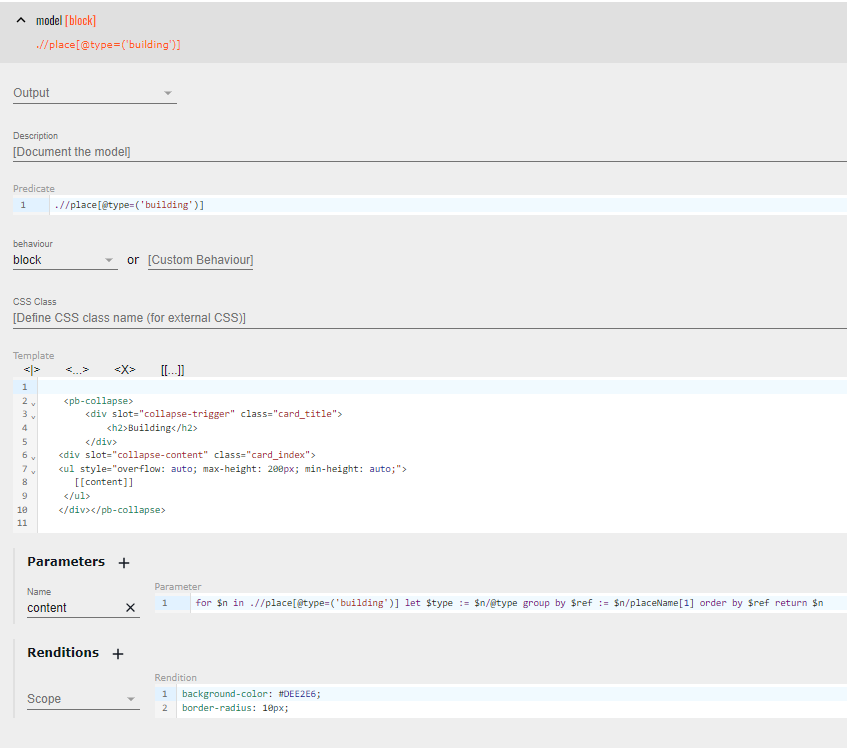
\includegraphics[width=0.75\linewidth]{schémas/building_places.png}
        \caption{Exemple de déclaration d’un élément dans l’interface graphique de l’ODD}
        \label{fig:schémas01}
    \end{figure}

Cependant, une ODD peut devenir inutile si elle n'est pas adaptée aux encodages spécifiques des fichiers XML que nous utilisons. DiScholEd contient sept collections provenant d'institutions différentes, et bien qu'elles respectent globalement les normes et directives de la TEI, certaines différences subsistent et peuvent perturber la conformité de l'ODD. Le problème ne viendra pas alors de TEI Publisher mais de notre ODD et/ou de l'encodage des corpus.

\subsection{Les templates HTML}

TEI Publisher, dans sa documentation, explique que pour produire une application, seules des compétences en HTML sont requises. C'est en effet nécessaire pour pouvoir utiliser les composants du \textit{Bundle} JavaScript (une librairie de balises HTML personnalisées). L'un des principes fondamentaux de TEI Publisher est de réutiliser et de partager les solutions ou idées des templates. Ainsi, les applications se ressemblent très souvent car elles proviennent du même ensemble de modèles, comme le montrent les figures suivantes (cf Figure \ref{fig:schémas02} et Figure \ref{fig:schémas03}):

\begin{figure}[H]
\centering
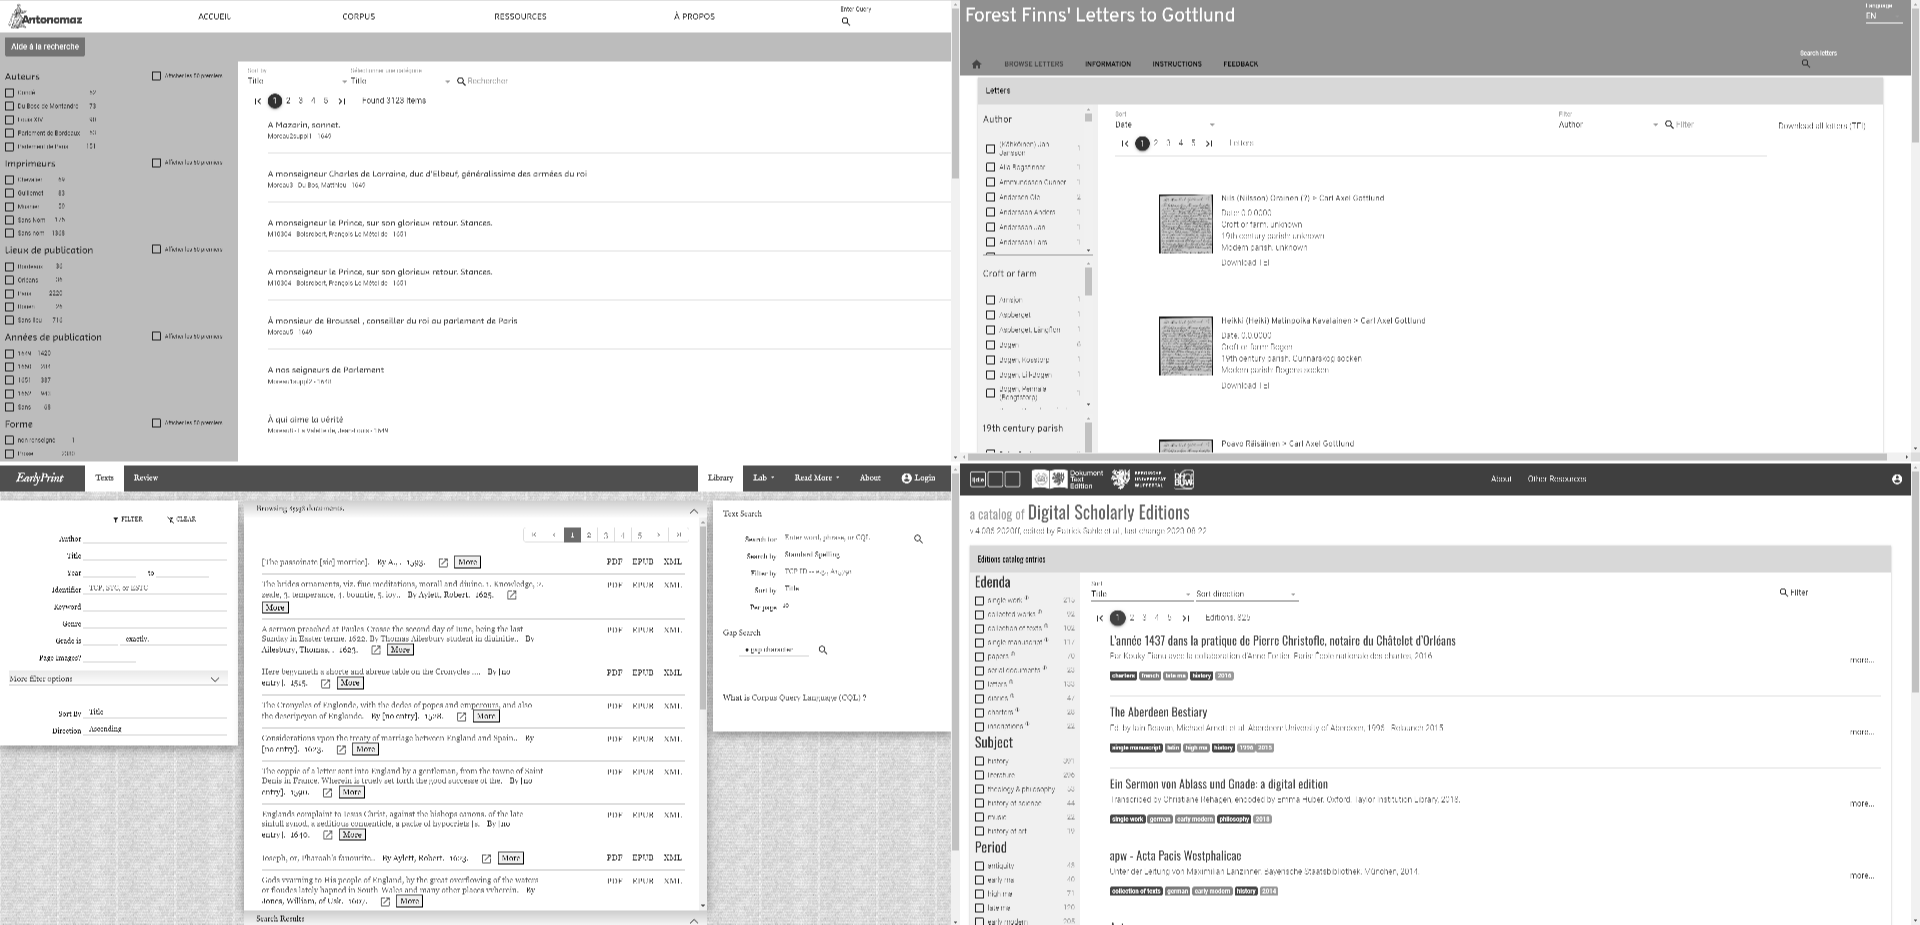
\includegraphics[width=1\linewidth]{schémas/4_webtei-modified.png}
\caption{Capture d'écran de 4 sites différents créés avec TEI Publisher (Antonomaz, Forest's Finn's Letter to Gottlund, Digital Scholarly Edition et EarlyPrint) }
\label{fig:schémas02}
\end{figure}

\begin{figure}[H]
\centering
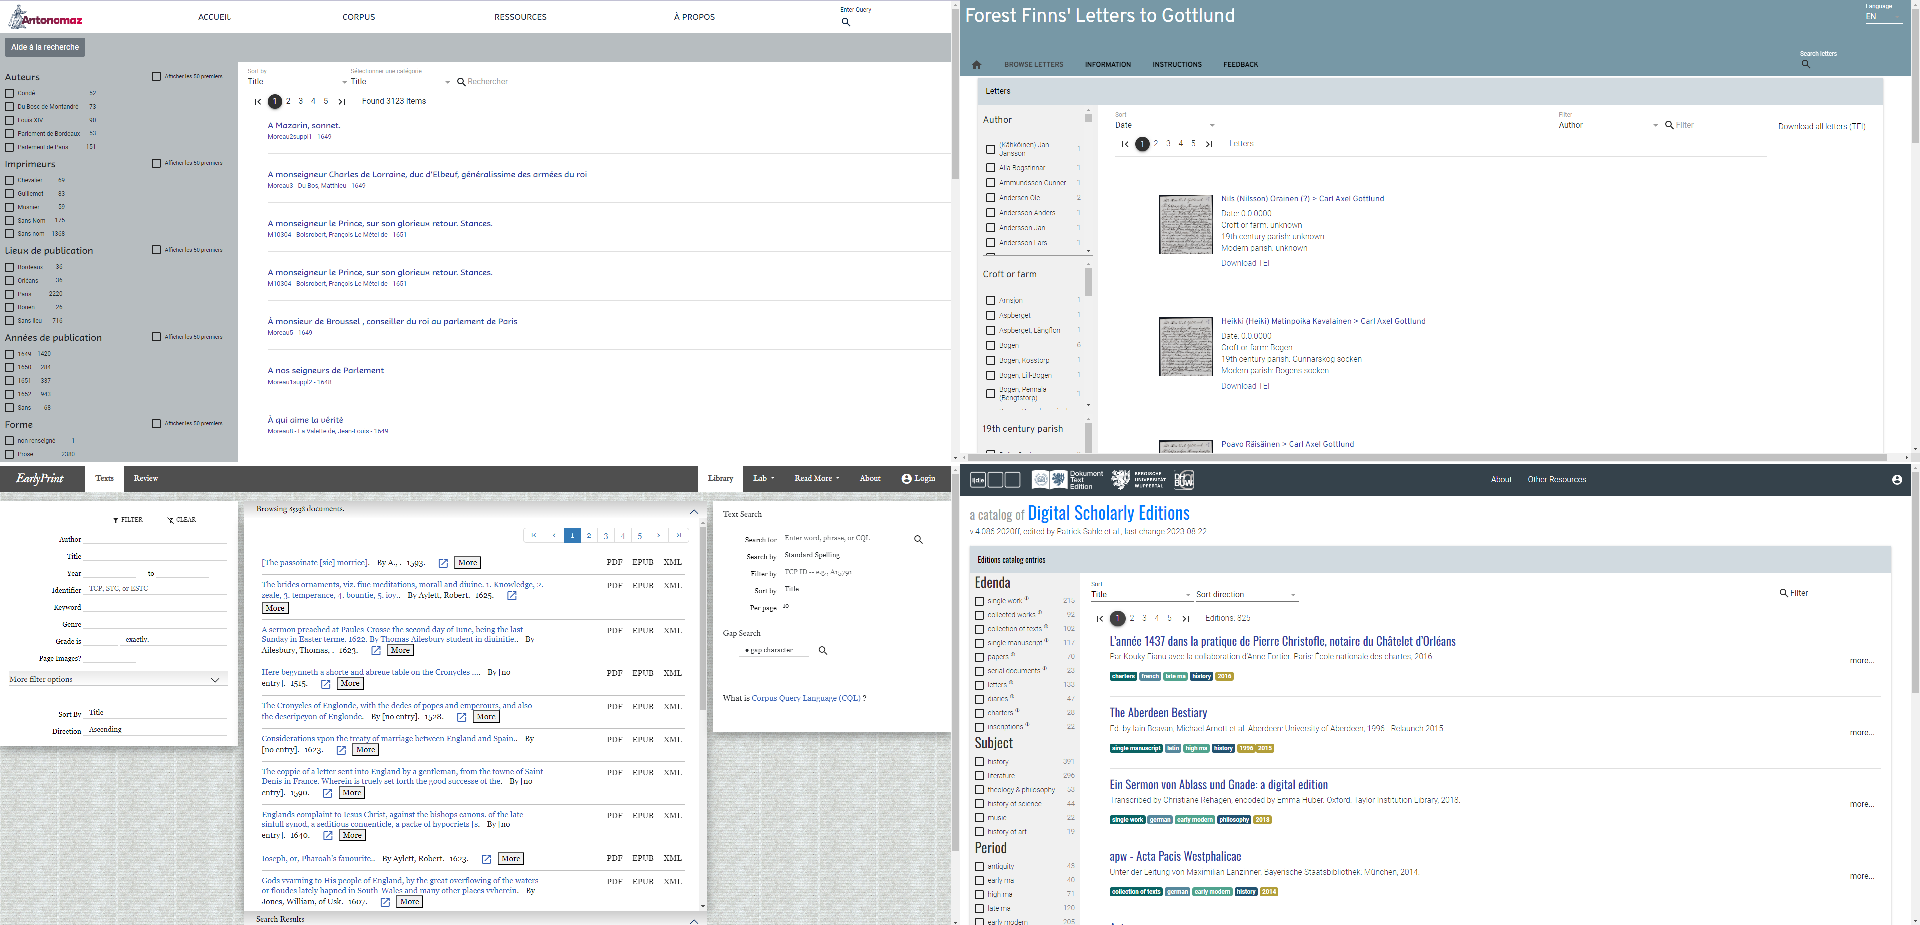
\includegraphics[width=1\linewidth]{schémas/4_webtei.png}
\caption{Capture d'écran des 4 sites avec leurs couleurs respectives (Antonomaz, Forest's Finn's Letter to Gottlund, Digital Scholarly Edition et EarlyPrint)}
\label{fig:schémas03}
\end{figure} 

La plupart de ces applications est souvent accessible sur Internet, avec une documentation complète de tous les composants disponibles sur \href{https://cdn.tei-publisher.com/@2.11.1/dist/api.html}{le site officiel}\footnote{\textit{TEI Publisher Webcomponents API}, URL: https://cdn.tei-publisher.com/@2.11.1/dist/api.html (visité le 29/08/2023)} de TEI Publisher.

TEI Publisher, en cherchant à offrir une grande liberté et à rendre la publication accessible aux non-codeurs, peut parfois générer des problèmes. Cette liberté peut désorienter les utilisateurs inexpérimentés, les amenant à prendre des décisions qui peuvent entraîner des erreurs. En d'autres termes, la flexibilité de TEI Publisher peut parfois se traduire par des erreurs, car elle permet aux utilisateurs de faire ce qu'ils veulent, même si cela ne correspond pas nécessairement aux meilleures pratiques en matière de développement.\\

Pour résumer, le projet DiScholed possède des corpus qui présentent tous un intérêt historique et a besoin d'un CMS pour les déployer sur Internet. Il existe beaucoup de CMS qui sont tous développés pour créer des applications bien spéciales. TEI Publisher, un CMS dédié aux éditions numériques et qui se veut accessible à tous, devrait être une solution pour notre projet. Le CMS parfait pour notre projet est assez libre pour nous permettre de mettre chaque corpus en avant et est assez restrictif pour nous évitez de détruire l'application. Nous avons identifié d'où pourraient provenir les \textit{bugs} générés par TEI Publisher, mais il nous faut maintenant examiner en détail ceux de DiScholed spécifiquement. En étudiant les \textit{bugs} de DiScholed, il sera alors possible de déterminer si TEI Publisher peut convenir à notre projet.
    \clearemptydoublepage
    \part{Le \textit{low-code} à l'épreuve des interventions techniques}
\setcounter{chapter}{0}

\chapter{La correction des erreurs}

Il existe trois catégories de défis présents sur DiScholEd (et sur toutes les applications web): 
\begin{itemize}[label=\textbullet]
\item Comment corriger les erreurs (\textit{bugs}) ?
\item Pouvons-nous ajouter de nouvelles fonctionnalités ?
\item Comment créer un \textit{design} personnalisé afin que notre application soit reconnaissable ?
\end{itemize}

Nous allons répondre à ces questions au travers d'études de cas et déterminer qui est en mesure de les résoudre. Notre objectif est de définir à qui s'adresse TEI Publisher. Pour rappel, il n'y a pas de développeur expérimenté sur le projet, mais normalement, TEI Publisher utilise le \textit{low-code}, ce qui devrait nous permettre de résoudre nos problèmes sans trop de difficultés.

Les erreurs signalées dans cette section sont générées par notre application et notre code, et non par TEI Publisher. Sur des projets avec moins de documents, ce type d'erreurs peut être facilement résolu, mais cela nécessite néanmoins une recherche approfondie. Nous allons expliquer comment TEI Publisher nous aide dans ce processus avec une étude de cas sur un \textit{bug} de l'application: les index.

\section{Le problème d'affichage des index}

C'est un \textit{bug} présent depuis le développement de DiScholEd. Dans notre application, chaque page de lettre doit afficher à droite du fac-similé un index. L'index comprend un bloc avec les entités nommées qui apparaissent dans le texte.
Il existe deux versions du \textit{bug}: l'un où le texte de la lettre s'ajoute à l'index (cf Figure \ref{fig:schémas04}) et l'autre où le texte apparait dans l'index même s'il n'y a pas d'entités nommées dans la lettre (cf Figure \ref{fig:schémas05}).

\begin{figure}[H]
  \centering
  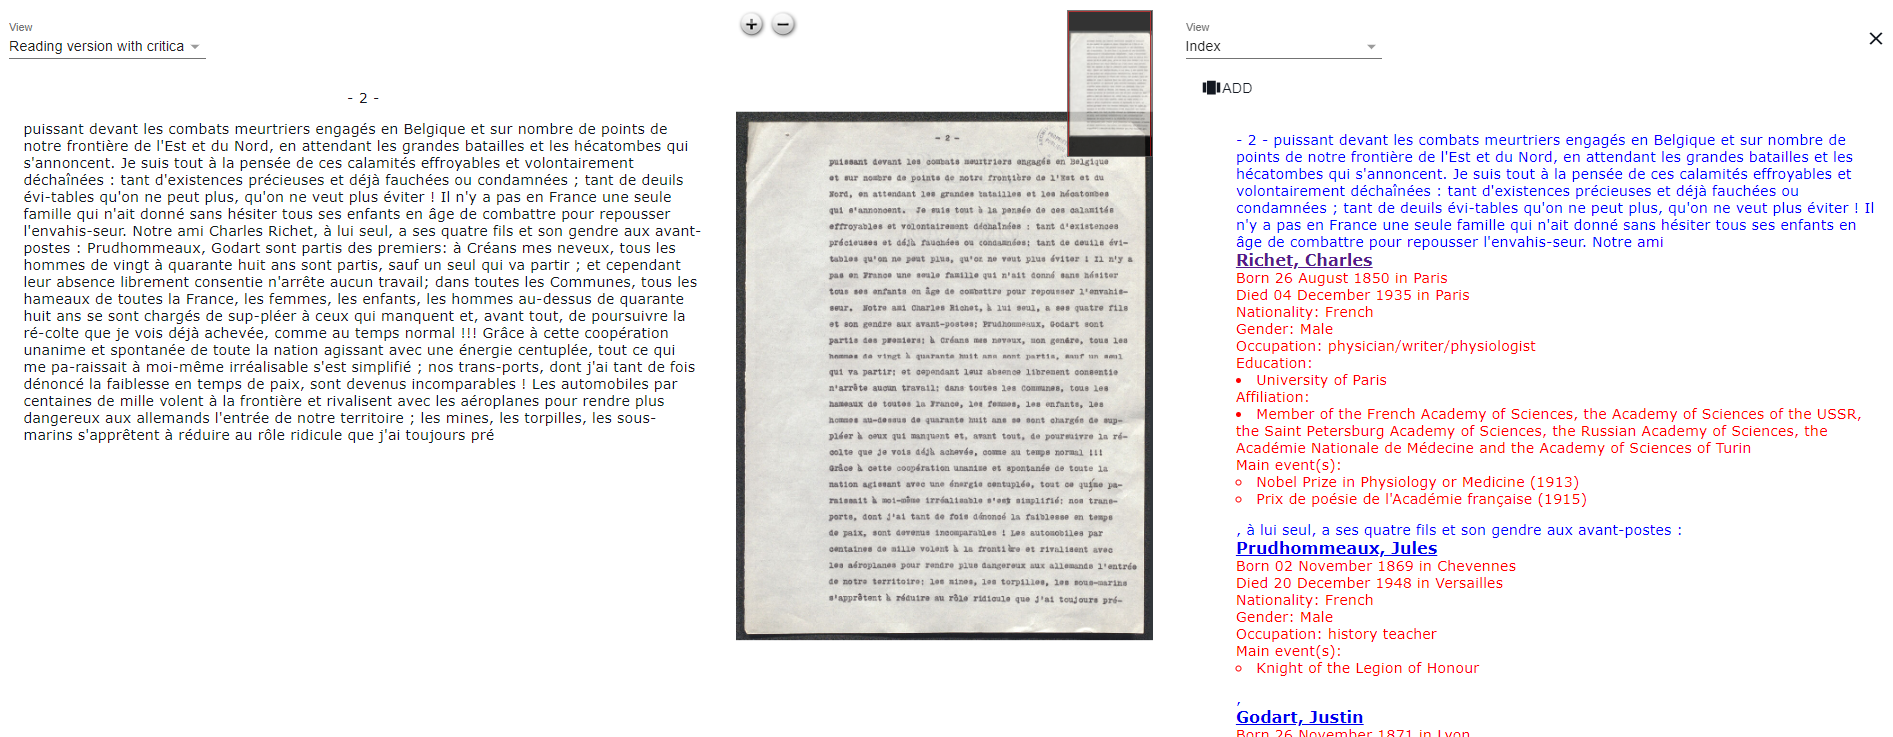
\includegraphics[width=1\linewidth]{schémas/facets text.png}
  \caption{Un exemple d'une lettre, avec le texte inattendu coloré en bleu et les informations d'index correctes colorées en rouge.}
  \label{fig:schémas04}
\end{figure}

\begin{figure}[H]
  \centering
  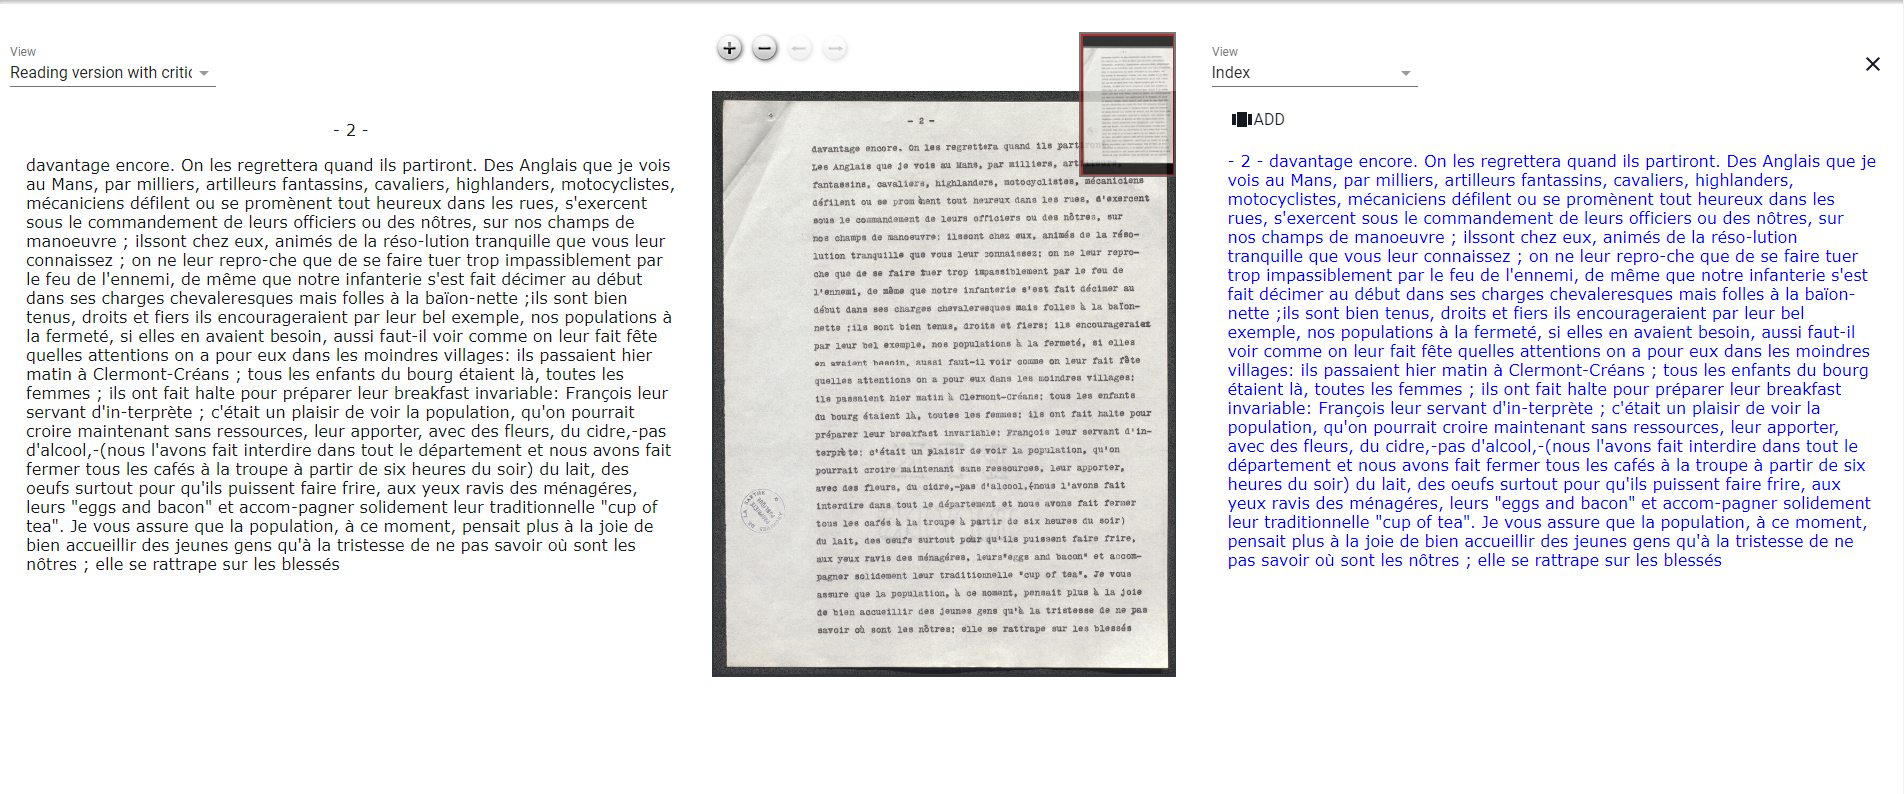
\includegraphics[width=1\linewidth]{schémas/facet_index.png}
  \caption{Un exemple d'une lettre, avec le texte inattendu coloré en bleu alors qu'il n'y a pas d'entités nommées.}
  \label{fig:schémas05}
\end{figure}

Le premier objectif est de comprendre ce qui génère ce problème. Le meilleur moyen est alors de dé-construire l'application et dans notre cas la page web. Il existe deux éléments qui contrôlent l'affichage des index: la page web et l'ODD. La page web appelle le document pour l'insérer dans la page, puis nous appliquons l'ODD au document. Si le problème venait de la page web et de l'HTML alors toutes les pages seraient défectueuses. Dans notre cas c'est donc l'ODD.  

\section{La résolution du problème}

Pour régler ce problème et grâce au \textit{low-code} de TEI Publisher nous pouvons utiliser l'interface graphique pour modifier notre ODD. La règle défectueuse est la balise <p>, qui nécessitait une modification de l'option qui était sur \textit{in-line} et devait être sur \textit{omit}. Cet ajustement a résolu avec succès le premier problème où le texte était dupliqué dans la section de l'index, même s'il n'y avait pas d'entités nommées dans le texte.

Toutefois, bien que le problème précédent ait été résolu, il restait à résoudre la présence du texte et de l'index dans la même section. Un examen plus approfondi a révélé que la balise <p> manquait à certaines pages, car elle faisait partie d'un paragraphe plus large englobant toute la page. Pour résoudre ce problème nous avons décidé d'ajouter des balises <p> d'ouverture et de fermeture accompagnées de commentaires justifiant leur présence. 

La prochaine étape consistait à identifier tous les fichiers où les balises <p> manquaient au sein de leurs sections <pb> (qui définit le début d'une nouvelle page). Dans ce but, un \nameref{script_python_p}(cf. Annexe \ref{script_python_p}) a été créé pour scanner les fichiers, enregistrer leurs noms de fichiers, et noter les balises <pb> correspondantes là où les balises <p> étaient absentes. Un fichier .csv a été généré pour suivre les fichiers problématiques. Ce script a été exécuté avec succès sur les 714 fichiers de l'application, révélant que 108 d'entre eux présentaient le problème identifié, comme nous pouvons le voir dans l’extrait du CSV présent dans la figure \ref{fig:schémas10} :

\begin{figure}[H]
\centering
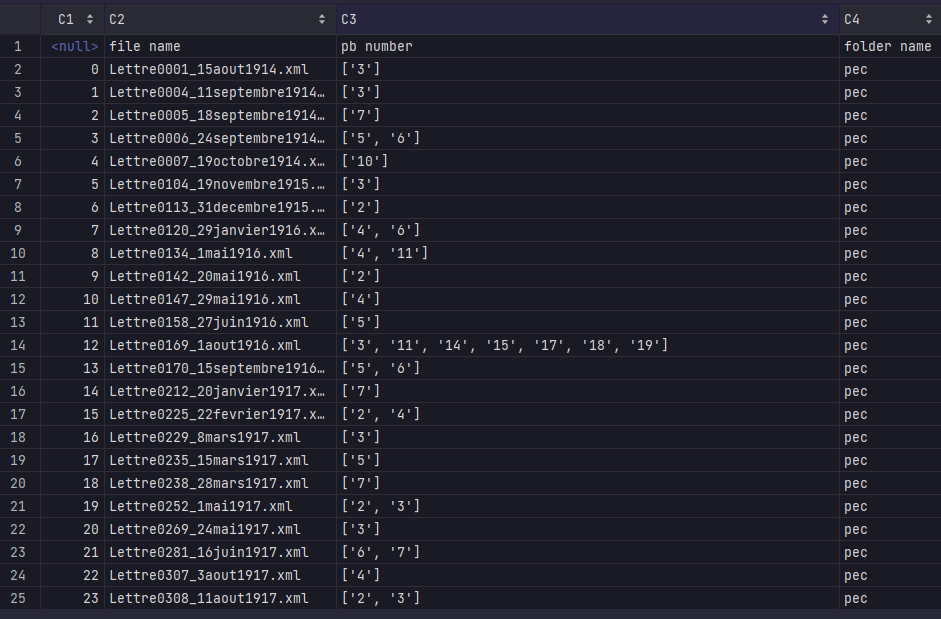
\includegraphics[width=0.75\linewidth]{schémas/script_python.png}
\caption{Le fichier csv qui regroupe tous les documents défectueux par nom de fichier, numéros de pages défectueuses, et nom de dossier.}
\label{fig:schémas10}
\end{figure}

Il a suffi alors pour régler le problème de modifier les fichiers défectueux. Pour ce deuxième cas de figure, TEI Publisher ne nous a pas aidés directement dans la résolution du problème. Nous avons dû trouver la source du problème par nous-mêmes, puis élaborer une solution adaptée à l'ensemble des corpus.

\section{Comment éviter ce bug pour la suite ?}

Le \textit{bug} apparaissait parce que la règle de l'ODD avait besoin d'une balise <p> pour comprendre qu'elle pouvait enlever le texte. Ce n'est pas une erreur qui provient de TEI Publisher, c'est l'un des défis de DiScholEd. En effet, avec autant de corpus, avoir une ODD qui prend en compte tous les cas de figure peut être très compliqué. Il existe deux manières d'éviter ce problèmes : forcer tous les encodages à respecter des règles strictes ou avoir une ODD qui arrive à prendre en considération tous les cas de figure possibles.

Ce \textit{bug} est chose courante dans la programmation et un développeur expérimenté va, avant même d'essayer de coder, réfléchir à tous les cas de figure possibles qui peuvent apparaître et qu'il faut alors prendre en compte. Néanmoins, sur 714 fichiers, c'est très probable d'avoir des oublis de balises. Le problème ne vient pas alors du CMS mais de l'encodage des fichiers. Les éditions numériques de la \textit{Bibliotheca Hertziana} ont par exemple pu éviter ce genre de problème en produisant une démo pour \og{}\textit{study the best way to make the content usable}\fg{}\footcite{epapers4200}.

Les problèmes de correction étaient nombreux, mais pour la plupart faciles à résoudre. Ils témoignent davantage d'une préparation qui n'a pas pris en compte tous les cas possibles d'un CMS défectueux. Pour résoudre ce problème, il n’est pas nécessaire d'avoir un développeur expérimenté, mais simplement la logique de développeur web (quelque chose d'accessible et rapide). 

Le plus souvent, il s'agissait de problèmes liés au HTML, une partie qui, comme l'avait annoncé TEI Publisher, doit être gérée par le développeur de l'application, qui doit avoir des compétences en HTML. La modification de l'ODD est complètement contrôlée par TEI Publisher et nous évite de commettre des erreurs grâce à une interface graphique simple à utiliser. D'ailleurs, des \href{https://www.youtube.com/watch?v=avRO-b2BwUI&ab_channel=wolfgangmm}{tutoriels}\footnote{\textit{TEI Publisher 3.0: Visual ODD Editor}, URL: https://www.youtube.com/watch?v=avRO-b2BwUI (visité le 29/08/2023)}, mis en place par TEI Publisher, sont disponibles pour nous apprendre à bien utiliser l'ODD.\\

Il est impossible pour TEI Publisher de détecter ce type de \textit{bug} ou de fournir des messages d'erreur, car la plupart d'entre eux sont des problèmes graphiques plutôt que des erreurs dans le code. 
Pour palier ces problèmes, TEI Publisher a mis en place une interface graphique, des tutoriels gratuits facilement accessibles, et met à notre disposition des canaux \href{https://app.slack.com/client/T012TH5TPJA/browse-channels/thread/C012YTJP5HB-1654605524.721479}{Slack\footcite{AllChannelsEeditiones}}pour communiquer avec les développeurs. Un autre avantage notable de TEI Publisher réside dans ses <pb-components>, qui nous permettent d'incorporer des éléments essentiels pour une navigation optimale dans notre application.

\chapter{Les nouvelles fonctionnalités de l'application}

\section{Le \textit{bundle} JavaScript}

Lors du développement d'applications web, les développeurs ont souvent recours à différentes bibliothèques, \textit{frameworks} et modules JavaScript pour ajouter des fonctionnalités et de l'interactivité à leurs sites web. Chacun de ces composants est généralement composé de plusieurs fichiers JavaScript. Cependant, le chargement de nombreux fichiers JavaScript séparés peut entraîner une augmentation des demandes réseau et des temps de chargement de page plus lents, ce qui impacte l'expérience globale de l'utilisateur. Pour atténuer ces problèmes, tous les fichiers JavaScript sont compactés dans un \textit{bundle}. TEI Publisher charge son \textit{bundle} depuis internet et donc ne peut pas être modifié, les balises spéciales que nous apporte le \textit{bundle} sont reconnaissables car elles contiennent le préfixe \og{}pb\fg{}, comme <pb-load>, <pb-browse> ou <pb-leaflet-map>.

Lorsque l'on utilise un CMS, l'intérêt est d'avoir accès à des fonctionnalités prêtes à l'emploi dès la création de l'application. C'est un avantage important des CMS restrictifs, l'objectif est d'obliger les utilisateurs à utiliser des éléments qui fonctionnent immédiatement. TEI Publisher, dans son \textit{bundle}, met en place des composants vitaux pour un site web d'éditions numériques, comme le <pb-browse> qui permet de parcourir une collection de documents avec des fonctionnalités de tri et de filtrage.\\

Au travers d'une étude de cas, nous allons expliquer les défis engendrés par la mise en place d'une nouvelle fonctionnalité, en l'occurrence <pb-timeline>, et comment TEI Publisher nous accompagne.

\section{Mise en place d'un composant: <pb-timeline>}

Une balise spéciale <pb-timeline> est utilisée pour afficher une chronologie de tous les fichiers d'une collection. Cette fonctionnalité est une nouveauté de la dernière version de TEI Publisher. Pour implémenter le <pb-timeline> dans la plateforme, une règle d'API personnalisée doit être créée. Pour <pb-timeline> un règle de l'API a été conçue pour renvoyer un objet JSON, où chaque propriété représentait une date ou le marqueur spécial \og{}?\fg{} indiquant des ressources non datées. Chaque entrée contenait une valeur correspondant à un nombre de ressources ou à un objet avec les propriétés \textit{count} et \textit{info} (les balises <a> qui font les liens vers les documents).

Alors que d'autres applications utilisaient une règle XQuery pour générer la chronologie dans un fichier XML, nous avons opté, pour l'utilisation d'un \nameref{script_python_timeline}(cf. Annexe \ref{script_python_timeline}) pour produire un fichier XML contenant les informations nécessaires, comme cela peut s’observer dans le fichier \nameref{xml_file_timeline}(cf. Annexe \ref{xml_file_timeline}). Ce fichier XML est ensuite transformé par l'API au format JSON attendu pour le <pb-timeline>.

Lorsque la page web se charge, l'élément <pb-timeline> appelle l'API et reçoit un fichier JSON, il crée alors un histogramme. Cet histogramme utilise le fichier JSON et, pour chaque année, il reçoit le nombre de documents correspondants. Il peut alors, pour chaque année, créer une barre qui, lorsqu'elle sera survolée avec la souris, pourra afficher les liens vers les documents l'année survolée.

\begin{figure}[H]
\centering
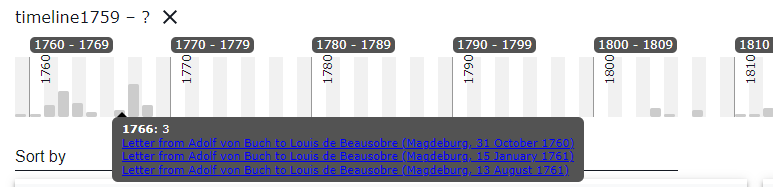
\includegraphics[width=0.75\linewidth]{schémas/timeline.png}
\caption{Un exemple d'un élément <pb-timeline> et de l'année 1766 du corpus \og{}Lettres et textes : Le Berlin intellectuel des années 1800\fg{}}
\label{fig:schémas06}
\end{figure}


\section{L'importance des éléments du CMS}

Pour réussir à utiliser les éléments propres à DiScholEd, il faut se référer à la documentation\footcite{TEIPublisherWebcomponents}. Les éléments de cette documentation sont spécifiques à TEI Publisher, ce qui constitue l'une des raisons qui pourraient nous inciter à opter pour ce CMS. Les éléments de TEI Publisher sont regroupés dans un ensemble appelé \textit{bundle}. Pour les intégrer dans notre application, il est nécessaire de se référer à la documentation, ou bien il est envisageable de télécharger des applications qui l'utilisent afin d'examiner et de comprendre comment ces éléments s'intègrent dans l'application. Par exemple, la timeline est utilisée par l'application : \href{https://www.briefedition.alfred-escher.ch/briefe/}{\textit{Briefe Editions} \footcite{EditionLettresEdition}}. 

La documentation peut être parfois lacunaire et les démos proposées ne sont pas fonctionnelles. C'est pourquoi pouvoir télécharger les applications est très important et permet de mieux comprendre comment l'élément fonctionne dans l'application. La mise en place de la \textit{timeline} demande des compétences élevées en développement et est l'un des éléments les plus compliqués à mettre en place. 

Il est aussi possible de s'affranchir du CMS et de faire comme pour le projet AGODA et \og{}\textit{implement components developed in the framework of TIME-US, and create new ones.}\footcite{puren:hal-03623351}\fg{}

Pour DiScholEd, l'utilisation du script Python pour créer les fichiers XML des timelines était obligatoire. En effet, les différences d'encodage dans les différents corpus nous ont empêché d'utiliser le XQuery officiel de TEI Publisher que \href{https://www.briefedition.alfred-escher.ch/briefe/}{\textit{Briefe Editions} \footcite{EditionLettresEdition}} utilise, par exemple.

La <pb-timeline> est un élément important : qui en plus d'améliorer le \textit{design} du site nous donne un aperçu rapide de la répartition dans le temps des documents. Néanmoins, sa mise en place demande de fortes connaissances en XQuery ou Python et est donc réservée à des développeurs.

Les éléments du \textit{bundle} jouent un rôle central dans la création d'une application de qualité, mais leur manipulation exige une solide expertise en informatique. Parfois, il est nécessaire de démonter d'autres applications pour parvenir à comprendre leur fonctionnement, faute de documentation adéquate. La mise en place de la \textit{timeline} n'est pas nécessaire pour les corpus suivants : le \og{}Journal des guerres napoléoniennes\fg{} et \og{}Ma Guerre 1914-1918\fg{}, qui ne comportent qu'un seul texte. En revanche, les cinq autres corpus contiennent généralement plus d’une centaine chacun, et avoir une répartition temporelle de tous les documents revêt une grande importance.

Certaines fonctionnalités de TEI Publisher sont trop complexes à mettre en œuvre pour les chercheurs. Cependant, ces éléments seraient moins pertinents pour leurs projets, car ils concernent souvent des ensembles de données plus restreints. TEI Publisher, bien qu'il se veuille accessible à tous, notamment aux chercheurs, n'en reste pas moins complexe à utiliser. Il est impossible de mettre en place des fonctionnalités complexes avec le \textit{low-code}, car cela requiert de la programmation en XQuery et une compréhension approfondie du fonctionnement de l'application. Pour les projets avec moins de documents, TEI Publisher permet effectivement de développer rapidement une application bien conçue. L'exemple du projet DiScholEd montre que la prestation d'un développeur ou de l'équipe de TEI Publisher est nécessaire pour développer l'application dans des conditions optimales.\\

Comme nous l'avons mentionné, TEI Publisher se situe quelque part entre la restriction et la liberté. Il convient aux projets qui n'exigent pas de fonctionnalités avancées, mais à mesure que le projet prend de l'ampleur, le besoin d'un véritable développeur devient de plus en plus crucial. Avec l'augmentation de la taille d'un projet, l'importance d'un bon \textit{design} devient cruciale.  

\chapter{L'amélioration de l'expérience utilisateur (UX)}

Les améliorations de l'application consistent en toutes les modifications apportées au \textit{design} de l'application. Par exemple, la mise en place des \textit{splash} est une amélioration de DiScholEd. L'UX (Expérience Utilisateur) d'une application web, lequel est étroitement lié à son \textit{design}, contrôle le ressenti global de l'utilisateur tout au long de son interaction avec l'application. L'UX englobe les défis d'accessibilités, d'esthétiques visuelles et d'ergonomies.

\section{Les fonds d'écran \textit{Splash} ou écrans de chargement}

Pour chaque collection, nous avons mis en place un arrière-plan d'écran de démarrage qui est une image de chargement utilisée comme arrière-plan. Lors du chargement d'une page, un écran de démarrage correspondant est appelé et affiché pendant que la page est en cours de chargement. Au début de mon stage, l'application n'avait pas d'écran de démarrage implémenté (cf Figure \ref{fig:schémas09}). Par conséquent, lors du chargement de la page, plusieurs informations aléatoires, telles que les langues disponibles dans l'application, étaient affichées au lieu d'un écran de démarrage spécifique.Nous avons alors mis à jour toutes les images des collections et des \textit{splash} avec des versions de meilleure qualité, enrichissant ainsi davantage l'expérience utilisateur (cf Figure \ref{fig:schémas07}-\ref{fig:schémas08}).

\newpage

\begin{figure}[H]
\centering
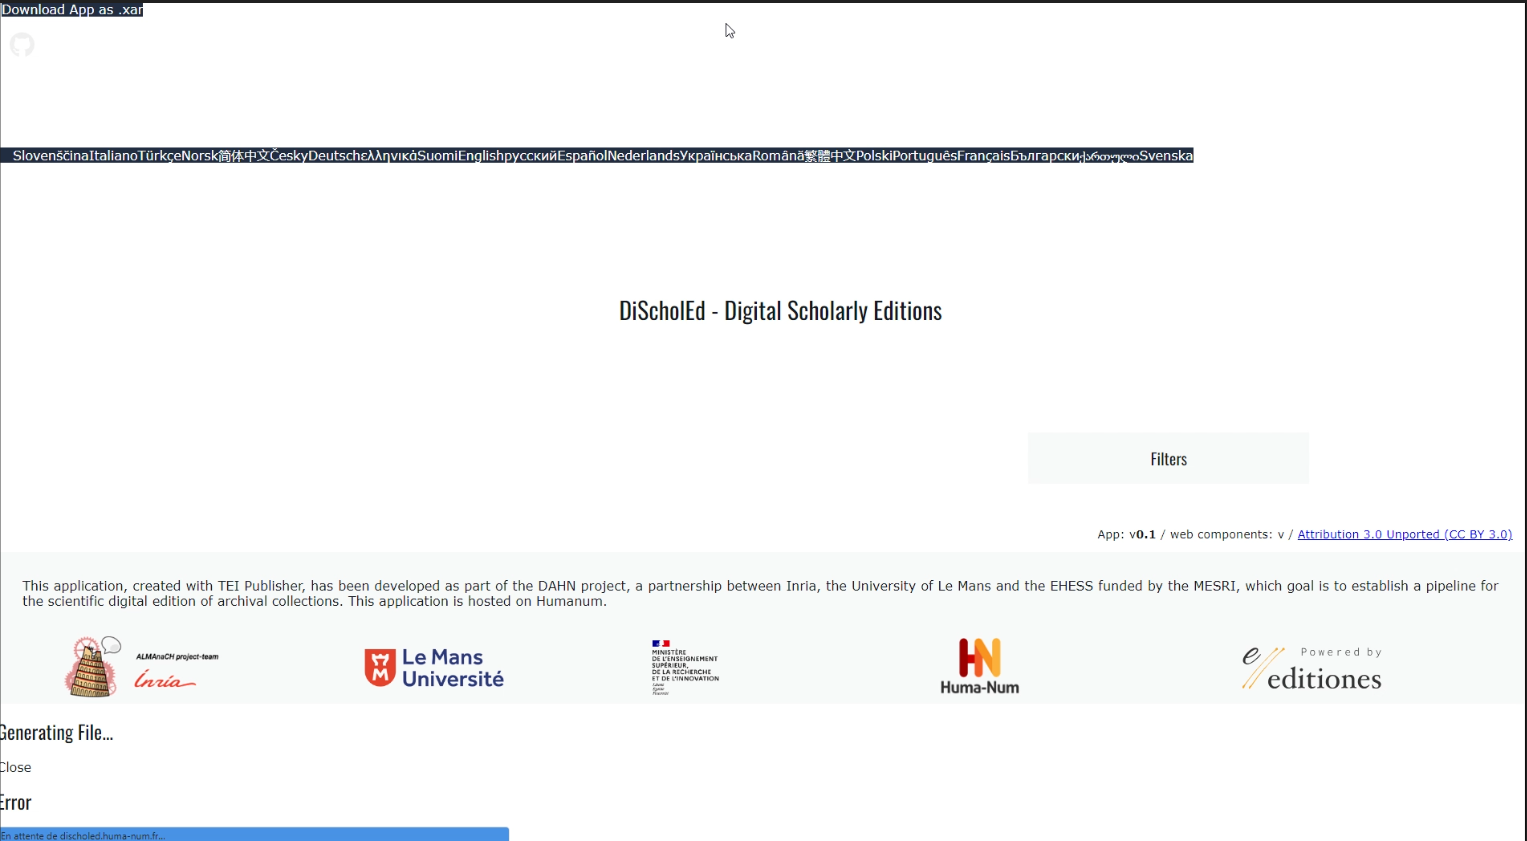
\includegraphics[width=0.75\linewidth]{schémas/old_splash.png}
\caption{Première version du \textit{splash} non fonctionnelle}
\label{fig:schémas09}

\centering

\includegraphics[width=0.75\linewidth]{schémas/new_splash.png}
\caption{Nouveau \textit{splash} de l'application}
\label{fig:schémas07}

\centering
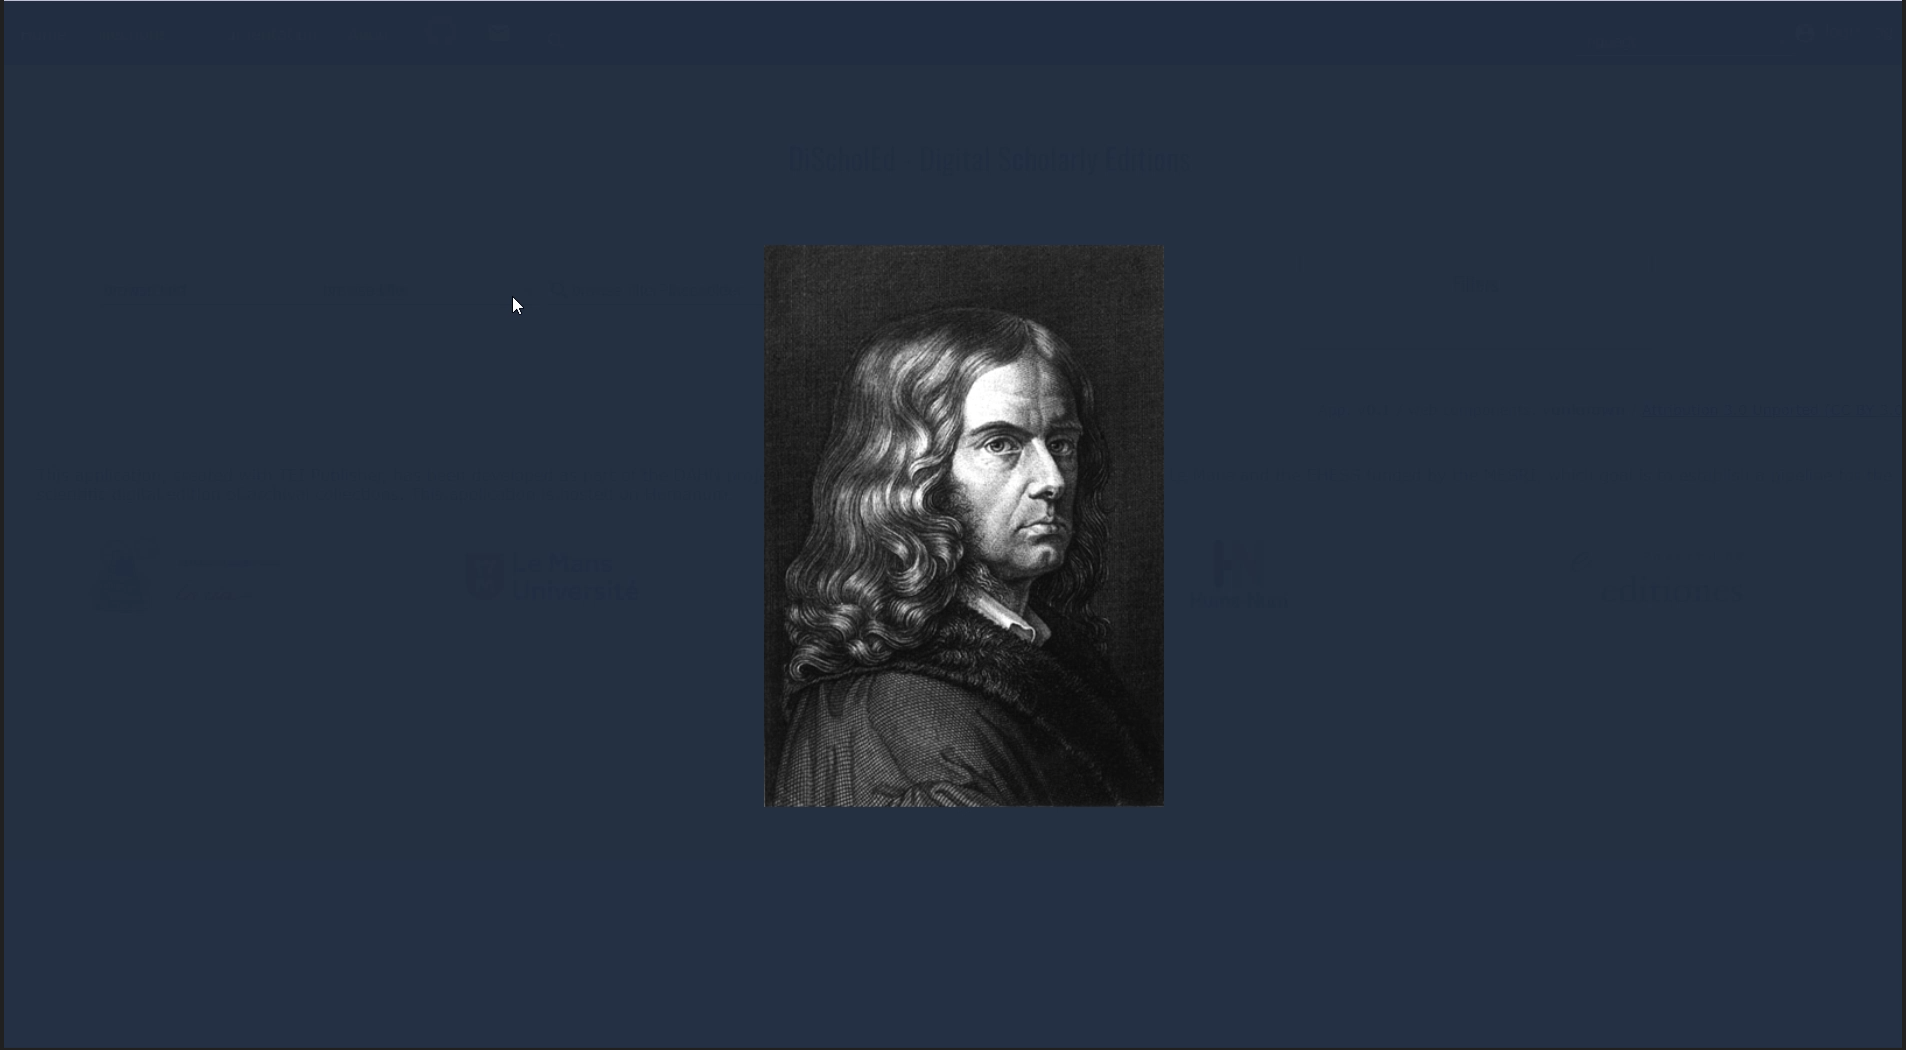
\includegraphics[width=0.75\linewidth]{schémas/new_splash_bi.png}
\caption{Nouveau \textit{splash} d'une collection}
\label{fig:schémas08}
\end{figure}

\section{L'importance du \textit{design} dans une application web}

Il est essentiel d'offrir une expérience utilisateur (UX) à la fois conviviale et mémorable. C'est la première impression que l'application laisse sur les utilisateurs, car elle constitue la façade de notre application et leur première interaction avec elle. Un site web doit être intuitif et facile à utiliser. DiScholEd, en tant que projet axé sur les éditions numériques, cible principalement un public de chercheurs. Une certaine connaissance en HTML est nécessaire pour la construction de notre site, car nous devons mettre en valeur sept corpus différents. Pour ce faire, nous avons mis en place plusieurs améliorations, notamment un carrousel des corpus sur la page d'accueil, une refonte du \textit{design} des pages de corpus et une amélioration de la qualité des images de présentation des corpus (cf Figure \ref{fig:schémas11}-\ref{fig:schémas13}).

\begin{figure}[H]
\centering
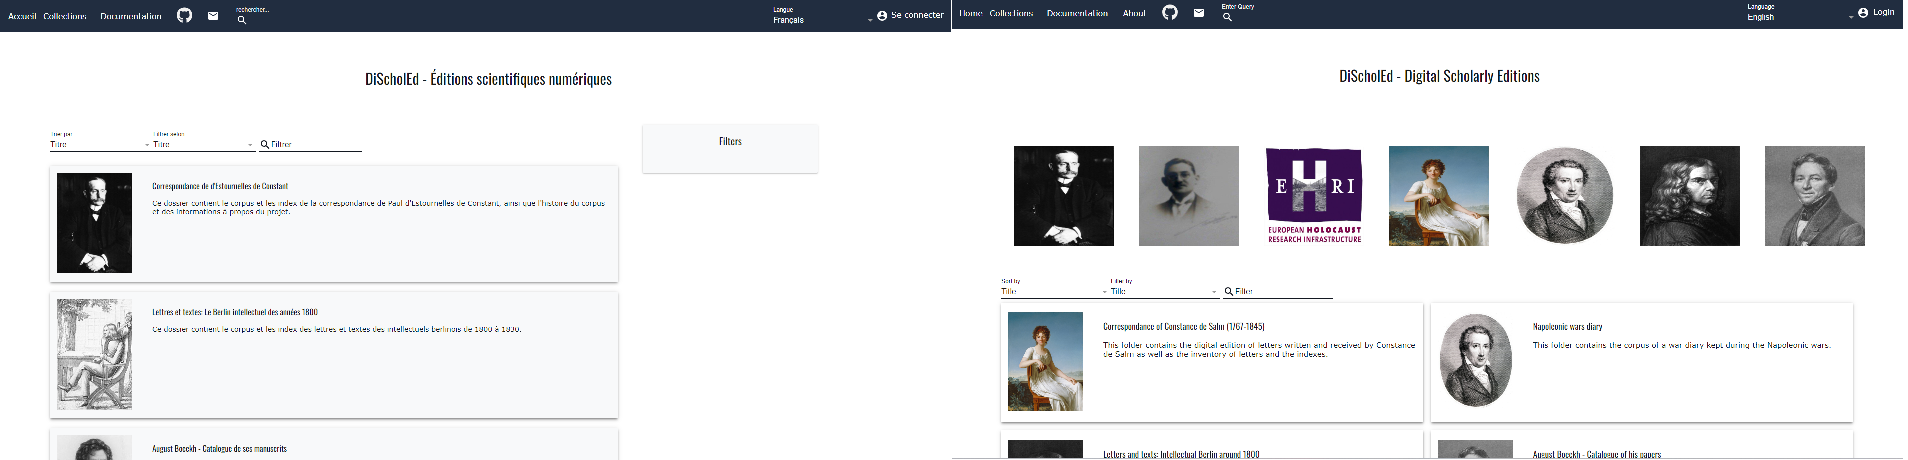
\includegraphics[width=1\linewidth]{schémas/carrousel.png}
\caption{ La page d’accueil sans le carrousel (gauche) puis avec (droite) }
\label{fig:schémas11}
\end{figure}

\begin{figure}[H]
\centering
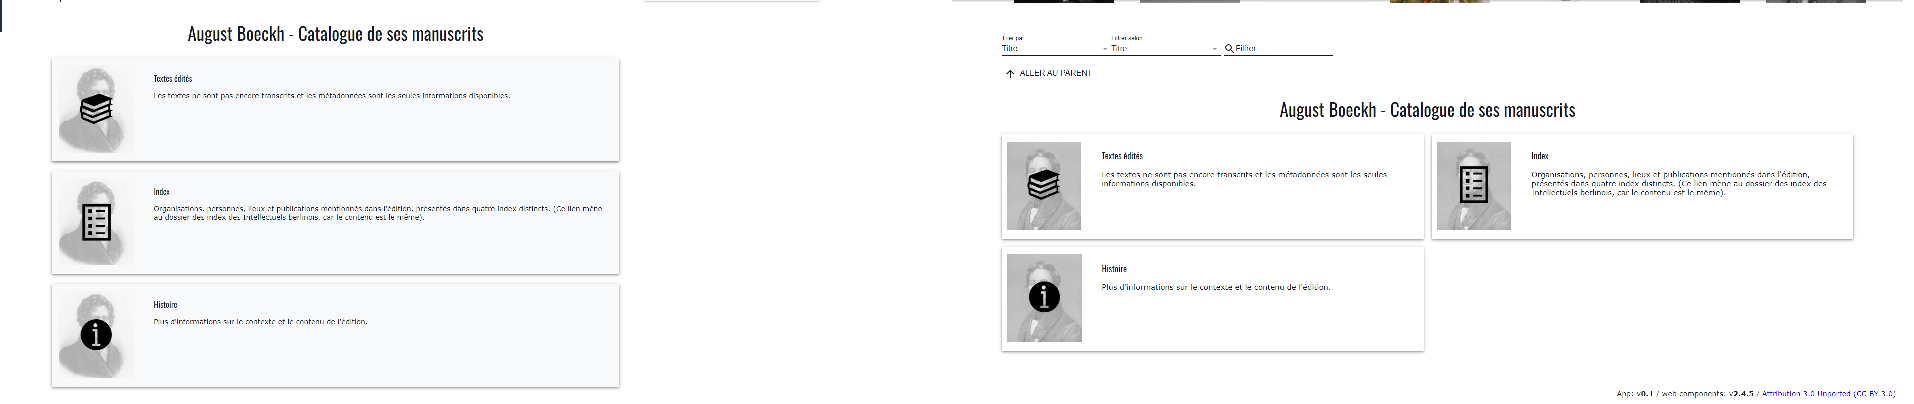
\includegraphics[width=1\linewidth]{schémas/page_corpus.png}
\caption{Les pages de corpus avant (gauche) puis après modifications (droite)}
\label{fig:schémas13}
\end{figure}

Pour mettre en place ces éléments de \textit{design}, seules des compétences de base en HTML sont nécessaires, à l'exception du carrousel, qui requiert des connaissances en JavaScript. TEI Publisher ne propose pas de fonction d'aide pour le HTML, car il nécessite une modification directe des fichiers HTML. Il existe de nombreux projets \textit{open source} qui peuvent servir de source d'inspiration pour des \textit{designs} intéressants, par exemple \href{https://teipublisher.com/exist/apps/vangogh/index.html}{Vincent van Gogh - The Letters
\footcite{VanGoghLetters}}. 

Cependant, il est important de noter que le \textit{design} d'un site web représente un véritable défi, qui devient d'autant plus complexe à mesure que la taille du site augmente. Par conséquent, il peut parfois être nécessaire de faire appel à un web \textit{designer}. L'avantage supplémentaire de travailler avec un web \textit{designer} est la possibilité de rendre le site adaptatif à différentes tailles d'écran, y compris les smartphones.

Un autre point pas encore abordé est le \textit{design} des éléments TEI Publisher qui proviennent du \textit{bundle}. Grâce à la documentation, nous avons à notre disposition des variables CSS pour modifier le \textit{design} des <pb-elements> (comme \textit{--pb-timeline-height}, qui permet de modifier la hauteur de la \textit{timeline}). Les variables mises à notre disposition ont été choisies par TEI Publisher et sont immuables. C'est l'une des raisons pour laquelle les sites TEI Publisher se ressemblent : le \textit{bundle} n'autorise pas une liberté assez grande pour pouvoir produire un \textit{design} propre à notre application. Le \textit{bundle} est contrôlé par TEI Publisher. Pour l'utiliser, il faut charger le fichier JavaScript depuis Internet, il est donc externe à notre application. Il existe une documentation dans la \href{https://faq.teipublisher.com/}{FAQ\footcite{FrequentlyAskedQuestions}} qui propose, à partir du \textit{bundle}, de modifier le \textit{bundle} en local et de développer ses propres éléments ou de modifier les existants. Le <pb-timeline> de DiScholEd devrait utiliser un \href{https://gitlab.inria.fr/dh-projects/discholed/-/blob/main/Pb-component-bundle/pb-timeline.js}{\textit{bundle} personnalisé\footcite{FilesMainDHprojects2023}}, mais nous n'avons pas réussi à le mettre en place pendant le stage. Le \textit{design} peut donc être modifié en profondeur mais demande de fortes connaissances en développement ou alors de faire appel à une société de \textit{design} comme les éditions numériques de la \textit{Bibliotheca Hertziana}: \og{}\textit{a complete re-\textit{design} with the support of a \textit{design} company}\fg{}\footcite{epapers4200}..\\

Nous avons choisi TEI Publisher parce que c'est un CMS dédié aux éditions numériques et qu'il est accessible aux non-développeurs. Cependant, à travers les différents problèmes de \textit{bugs}, la mise en place de nouvelles fonctionnalités et l'amélioration générale de l'application, il semble que de nombreux problèmes apparaissent, soulevant de nouveaux défis et questionnements. Comme nous l'avons également observé, plus notre application est grande, plus les problèmes sont fréquents et difficiles à résoudre. Chaque nouveau corpus ajoute des documents avec des encodages qui ne sont parfois pas adaptés à notre ODD et demande une refonte d'une partie de l'ODD spécialement pour ce corpus. Le \textit{low-code} nous permet d'utiliser des balises personnalisées du \textit{bundle} et de l'interface graphique de l'ODD. Cependant il est nécessaire, vu la taille de notre application, d'aller directement dans les fichiers pour modifier manuellement le \textit{design} et l'ODD. Nous pouvons alors émettre l'hypothèse que le \textit{low-code} devient donc obsolète à mesure que l'application grandit, cependant son obsolescence est due à deux facteurs : une variation de l'encodage des fichiers et un \textit{bundle} qui restreint fortement le \textit{design} général. 
    \clearemptydoublepage
    \part{Les améliorations possibles de TEI Publisher et DiScholEd}

\setcounter{chapter}{0}

\chapter{L'audience cible de TEI Publisher}

\section{Un entre-deux entre chercheur et programmeur} 

Comme nous l'avons vu, TEI Publisher est un CMS à la fois restrictif et ouvert. L'équilibre qu'il offre permet de créer rapidement une application, mais il peut aussi entraîner une certaine similitude avec d'autres applications. Les avantages du low-code, cependant, peuvent parfois freiner le travail d'un programmeur.

Les problèmes que nous avons rencontrés sont soit inhérents au CMS, soit provoqués par celui-ci. Pourtant, l'un des avantages des CMS réside dans la gestion des \textit{bugs}, car on utilise normalement un produit déjà fonctionnel qui ne nécessite pas de codage supplémentaire.

Même si TEI Publisher se veut accessible aux chercheurs n'ayant pas de compétences en programmation, il peut s'avérer difficile de créer une application à la fois fonctionnelle et originale. 

Ainsi, un chercheur qui opte pour TEI Publisher choisira une application fonctionnelle, ce qui peut être la meilleure solution. Il vaut mieux avoir une application simple et entièrement fonctionnelle plutôt qu'une application avec une identité propre mais des problèmes techniques. La problématique liée au choix de TEI Publisher dépend donc des compétences techniques du développeur/chercheur ainsi que de l'envergure du projet.

\section{Un CMS pour des projets avec peu de documents}

TEI Publisher est une solution idéale pour les chercheurs qui ne maîtrisent pas la programmation et souhaitent rapidement et facilement créer leur propre application web. Tout au long de ce mémoire, nous avons abordé à plusieurs reprises le défi de la limitation imposée par TEI Publisher. Cependant, il est envisageable de créer une application qui se démarque en utilisant TEI Publisher, mais cela nécessiterait une solide expertise en programmation. Cela dit, avec de telles compétences en programmation, il est tout à fait possible de créer une application à partir de zéro, sans avoir recours à un CMS.

\section{Exemples d'autres projets fonctionnels d'éditions numériques}

\subsection{Édition électronique des œuvres de Jean-Joseph Rabearivelo}

Jean-Joseph Rabearivelo (1901-1937) était un poète et écrivain malgache. Il est né le 4 mars 1901 à Tananarive, qui était alors une colonie française. Sa poésie, influencée par la culture malgache traditionnelle ainsi que par la littérature française, a été acclamée pour sa richesse linguistique, sa musicalité et son exploration de thèmes tels que l'amour, la nature et la quête d'identité. Ses œuvres ont contribué à élever la langue malgache au rang de langue littéraire et à la faire reconnaître comme un moyen d'expression artistique. Malheureusement, malgré son talent et sa contribution à la littérature, Jean-Joseph Rabearivelo a connu des difficultés personnelles et des problèmes de santé mentale. Il est décédé tragiquement le 22 juin 1937, laissant derrière lui un héritage littéraire durable.

Le corpus Rabearivelo a donné matière à une \href{https://www.cnrseditions.fr/auteur/jean-joseph-rabearivelo/}{édition papier}\footnote{https://www.cnrseditions.fr/auteur/jean-joseph-rabearivelo/} (2010-2012), cette édition est publiée dans la collection « Planète libre » de CNRS Éditions. Clément Plancq (LATTICE-CNRS) a ensuite encodé au format XML/TEI le corpus Rabearivelo en vue d'une édition numérique avec TEI Publisher.\footcite{riffard:halshs-03979331}

L'application fonctionne très bien ; elle se compose seulement de 4 documents et est en développement. Le \textit{design} utilise le \textit{bundle} de TEI Publisher. C'est un exemple d'une application avec peu de documents qui, au détriment d'un \textit{design} original, a fait le choix d'une application fonctionnelle.

\subsection{\textit{Travel Reports of a Pioneer}}

Johann Conrad Fischer (1773-1854) est une figure emblématique de son époque, un pionnier de la Révolution Industrielle, et le fondateur de GF, une entreprise qui allait devenir l'un des acteurs majeurs de l'industrie européenne. Sa vie et ses réalisations sont remarquables à bien des égards, et sa contribution à la compréhension de son temps est inestimable.

Né en 1773, Johann Conrad Fischer a vécu à une époque charnière de l'histoire, celle de la Révolution Industrielle. Dès son plus jeune âge, il a montré un intérêt marqué pour les avancées technologiques et industrielles de son temps. À l'âge de 19 ans, il a entrepris un voyage d'apprentissage qui l'a conduit à parcourir plus de 30 000 kilomètres, une expérience qui l'a profondément marqué.

Fischer a publié les notes de neuf de ses voyages dans sept journaux entre 1816 et 1853. Bien que les manuscrits originaux de ces premières publications aient disparu, en 1951, l'historien Karl Schib a réalisé la seule édition critique de tous les journaux de Fischer à ce jour.

En 2023, \textit{the Iron Library} (URL : \href{https://www.eisenbibliothek.ch/en.html}{https://www.eisenbibliothek.ch/en.html}) a réalisé une édition numérique des textes en allemand, accompagnée de leur traduction en anglais pour célébrer les 250 ans de Fischer. Pour ce faire, ils ont choisi d'utiliser TEI Publisher.

La réalisation de cette application a nécessité l'implication du développeur Lars Windauer, de l'entreprise Jinntec spécialisée dans les éditions numériques et TEI Publisher. Cet exemple illustre parfaitement comment une application peut exploiter TEI Publisher sans être contrainte par un \textit{design} préétabli, mais requiert une aide technique. De plus, à l'instar du projet AGODA, des fonctionnalités propres à l'application ont été développées, notamment la possibilité de visualiser le trajet décrit dans le chapitre sur une carte en même temps que la lecture.

\chapter{Les choix possibles de TEI Publisher}

\section{CMS restrictif et le passage au \textit{no-code}}

Un des moyens pour transformer TEI Publisher en un CMS accessible et facile d'utilisation pourrait être de passer au \textit{no-code}. Le \textit{no-code}, contrairement au \textit{low-code}, restreint tout accès au code.

Par exemple, \href{https://fr.wordpress.org/}{\textit{WordPress}\footcite{WordPress}} fonctionne avec le no-code et utilise des blocs pour créer une application web. Toutes les fonctionnalités sont contrôlées par le CMS et empêchent les \textit{bugs} majeurs.
Même si cette idée semble intéressante, il faudrait développer toute l'interface graphique pour contrôler les blocs. La tâche est gigantesque et demanderait plusieurs années de développement.

De plus, passer au \textit{no-code} pourrait bénéficier à des chercheurs qui ne veulent pas coder, mais ont-ils vraiment besoin de passer au no-code ? La plupart des applications qui semblent avoir été créées pour de petits corpus par des chercheurs fonctionnent parfaitement, comme: \href{https://rabearivelo.huma-num.fr/exist/apps/jjr/index.html}{Jean-Joseph Rabearivelo\footcite{JJR}} ou \href{https://teipublisher.info/exist/apps/TraveLab/index.html}{TraveLab\footcite{TraveLab}}.

\section{Un \textit{design} universel} 

Un \textit{design} universel ne se limite pas à l'utilisation du \textit{no-code}, mais plutôt à la possibilité d'utiliser des modèles (\textit{templates}) déjà conçus. Ainsi, toutes les applications auraient une apparence identique, mais elles fonctionneraient parfaitement. On pourrait également envisager que le \textit{design} soit développé pour fonctionner sur d'autres plateformes, telles que les \textit{smartphones}. Un autre avantage consisterait à établir une norme permettant aux utilisateurs de reconnaître le site et de l'utiliser immédiatement.

Dans son article, Elena Pierazzo défend également l'idée d'un CMS qui serait accessible à tous les chercheurs. Elle le décrit ainsi : \og{}\textit{scholar to be able to annotate their texts in a suitable format and to choose among several displaying options}\fg{}\footcite{epapers4200}.

Pour réussir à développer ce CMS avec un \textit{design} fonctionnel, adaptable et simple, imposé qui éviterait tous les problèmes liés au \textit{design}, il faudrait alors standardiser tous les documents.

\section{L'encodage des documents}

Pourquoi y a-t-il autant de \textit{bugs} sur DiScholEd ? Comme nous l'avons vu à travers tous les problèmes, la principale raison provient des encodages des corpus. Il semblerait d'ailleurs qu'aucune application TEI Publisher ne possède plusieurs corpus au sein de la même application. Les sept corpus font de DiScholEd une application importante et constituent un exemple de la manière dont TEI Publisher gère les applications avec plusieurs corpus. Même si les encodages respectaient la TEI, des coquilles ou des erreurs ralentissaient le développement et le déploiement de l'application. En septembre 2023, l'application fonctionne parfaitement.

\chapter{Le futur de Discholed}

\section{La mise en place des ODD}

En mettant en place une ODD pour chaque corpus, il serait possible de résoudre rapidement les problèmes survenus. Néanmoins, il faudrait découper notre ODD, qui est composée de milliers de lignes, pour retrouver les règles propres à chaque élément. Pour tous les nouveaux corpus, il faudrait aussi recréer une ODD complète et reprendre toutes les règles déjà mises en place. L'objectif derrière la création des ODD serait de pouvoir gérer tous les cas de figure des encodages des corpus. Il faudrait aussi reprendre sept ODD si on découvre un \textit{bug} dans notre application.\\

La création des ODD semble être une solution très chronophage mais qui pourrait nous permettre de régler les \textit{bugs} spécifiques à certain corpus rapidement. Les ODD pourraient alors fonctionner avec des encodages qui normalement ne fonctionneraient pas pour notre application. Néanmoins, il semble sûrement plus intéressant de vérifier les encodages plutôt que de faire du cas par cas. La mise en place de GitHub Actions pourrait remédier à ce problème.

\section{Les GitHub actions}

Sur le dépôt GitHub de DiScholEd, un flux de travail GitHub Actions a été développé dans le but de vérifier les encodages des fichiers avant leur dépôt sur GitHub. GitHub Actions est un système d'automatisation basé sur des événements. Il réagit aux événements survenant dans un GitHub, tels que les validations de code, les demandes de fusion, les créations de nouvelles versions, et bien d'autres. Lorsqu'un événement déclenche un flux de travail (workflow), GitHub Actions exécute une série de tâches définies par le développeur. À partir de septembre 2023, pour ajouter un nouveau corpus sur DiScholEd, il est nécessaire de faire une demande de fusion dans le dépôt GitHub de DiScholEd.

À chaque demande de fusion, le \nameref{git_action}(cf. Annexe A.4) s'active. Il utilise alors un script Python pour vérifier si les documents que l'on essaie de fusionner correspondent à notre ODD. S'il détecte une erreur (cf Figure \ref{fig:schémas14}), il renvoie un message d'erreur, interrompt la demande de fusion et crée une \textit{issue} avec une explication détaillée (cf Figure \ref{fig:schémas15}).

\begin{figure}[H]
\centering
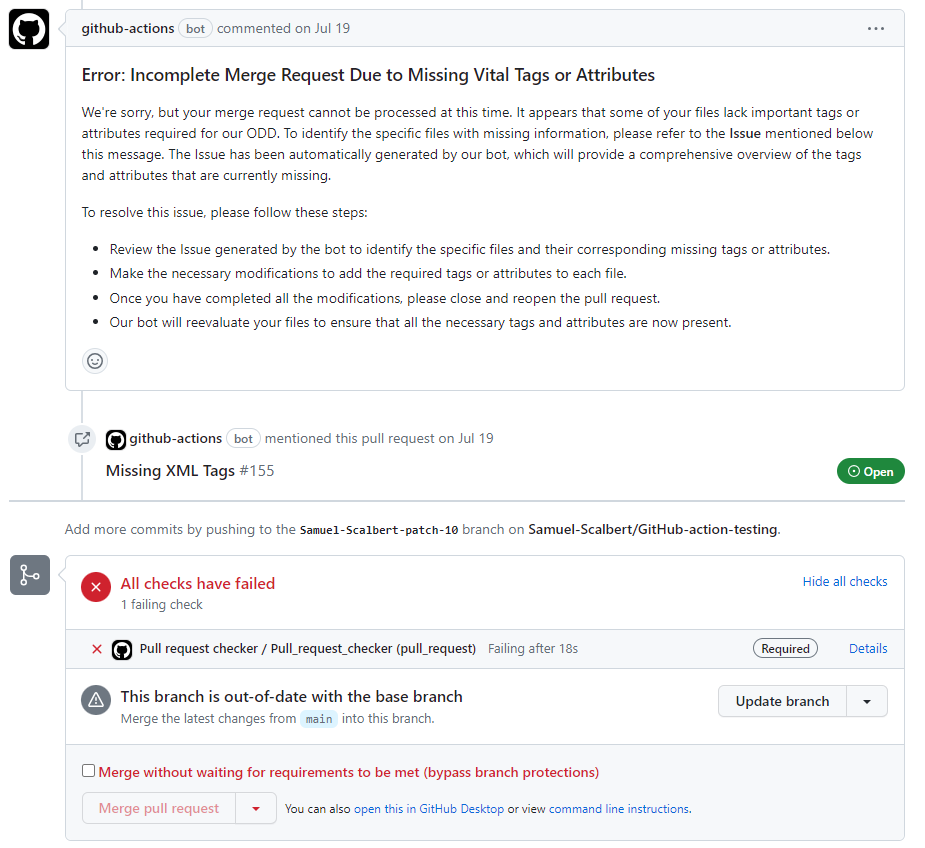
\includegraphics[width=0.75\linewidth]{schémas/gitaction_pr.png}
\caption{Exemple d'une demande de fusion refusée par GitHub Actions}
\label{fig:schémas14}
\end{figure}

\begin{figure}[H]
\centering
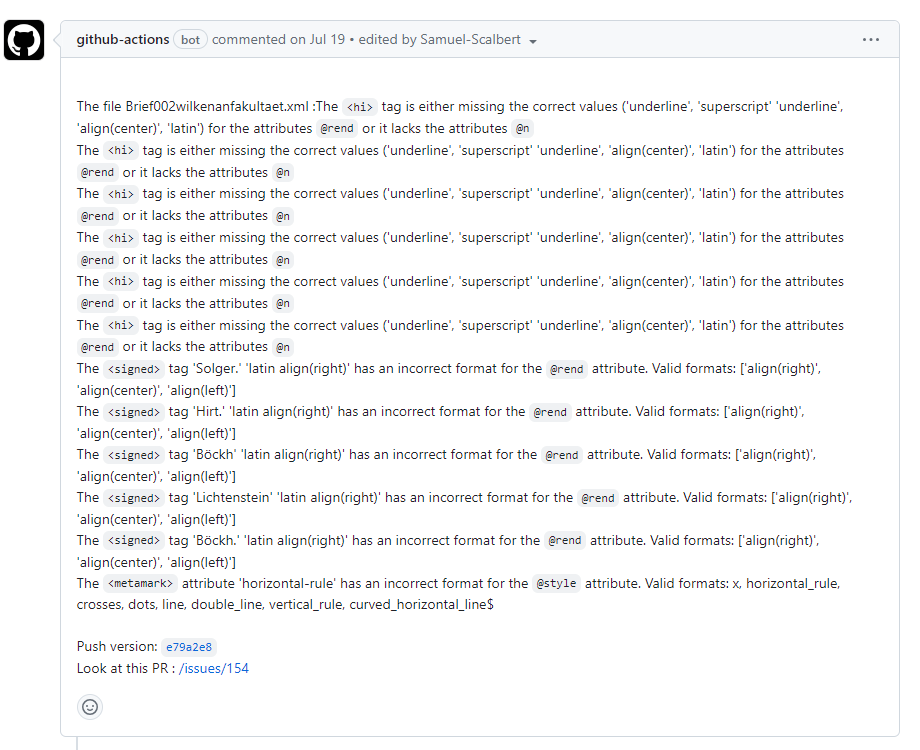
\includegraphics[width=0.75\linewidth]{schémas/gitactions_issue.png}
\caption{Exemple d'une \textit{issue} créée par GitHub Actions}
\label{fig:schémas15}
\end{figure}

Ce GitHub Action permet de vérifier rapidement et facilement si l'encodage du corpus correspond à notre ODD, évitant ainsi de nombreux problèmes. De plus, elle offre la possibilité à toute personne souhaitant soumettre son corpus à DiScholEd de vérifier directement son encodage, sans avoir à attendre l'approbation d'un membre de l'équipe DiScholEd.\\

Le dernier problème, après l'encodage des fichiers, était le \textit{design} de notre application.

\section{Un \textit{bundle} spécifique pour Discholed}

Nous avons souvent évoqué le \textit{bundle} de TEI Publisher et expliqué qu'il apporte des fonctionnalités essentielles, mais qu'il limite le \textit{design} général de l'application.

Il est possible de créer son propre \textit{bundle} à partir de celui disponible sur le \href{https://github.com/eeditiones/tei-publisher-components}{GitHub}\footnote{URL : https://github.com/eeditiones/tei-publisher-components} de TEI Publisher. Un \textit{bundle} spécialement développé pour notre application pourrait résoudre tous nos problèmes, mais cela nécessite une solide expertise en développement. Le seul inconvénient alors serait que notre \textit{bundle} ne recevrait plus les mises à jour.

En effet, en utilisant une version modifiée du \textit{bundle}, il faudrait le charger non plus depuis Internet, mais à partir des fichiers de l'application. Ainsi, notre \textit{bundle} ne serait plus mis à jour, nos éléments fonctionneraient, mais nous perdrions les nouvelles fonctionnalités développées par TEI Publisher et les correctifs de \textit{bugs}.

    \clearemptydoublepage
    \chapter*{Conclusion}
\addcontentsline{toc}{chapter}{Conclusion}

Ce mémoire a pour objectif de présenter le travail accompli au cours du stage, ainsi que de réfléchir aux causes des problèmes rencontrés, à l'implémentation de nouvelles fonctionnalités et au \textit{design} de notre application. Cette réflexion nous a permis de mieux appréhender les avantages et inconvénients de l'utilisation de TEI Publisher.

TEI Publisher propose des fonctionnalités avancées pour la gestion de documents XML. Grâce à une approche en \textit{low-code}, il offre la possibilité à des chercheurs peu familiarisés avec l'informatique de publier leurs éditions de manière aisée et rapide, et permet aussi aux développeurs de créer des applications complexes. Mais pour les chercheurs, les restrictions qu'impose TEI Publisher vont rapidement imposer : soit de recruter un développeur pour créer une application spécifique, ou alors de se contenter d'une application simple et fonctionnelle mais limitée dans le \textit{design}. Pour certains développeurs, ils préféreront créer leur propre application.

En privilégiant l'accessibilité pour tous, TEI Publisher se révèle être une solution pertinente pour les éditions numériques. Néanmoins, à travers l'analyse de cas d'études et les correctifs apportés à l'application, il apparaît que de nombreux problèmes subsistent. Ces problèmes ne sont pas inhérents au CMS lui-même, mais résultent d'erreurs dans l'encodage des documents XML. Heureusement, nous avons réussi à les résoudre tous sans compromettre l'intégrité de l'application. La correction de ces problèmes a également permis de mieux comprendre leur origine et d'envisager une solution pour les prévenir : l'utilisation de GitHub Actions.

DiScholEd est une application originale qui cherche à rendre accessible sept corpus malgré leurs différences, ce qui soulève de nouveaux défis et met en lumière les limitations de TEI Publisher. Il est ardu, voire impossible, pour un CMS de s'adapter à tous les projets. Bien que TEI Publisher aspire à être accessible et ouvert à tous, s'il reste un outil utile et novateur pour les éditions numériques, qui n’est cependant pas exempt de faiblesses.
	\clearemptydoublepage
 
	%les annexes
    \backmatter
	\part*{Annexes}
\addcontentsline{toc}{part}{Annexes}
\appendix
\renewcommand{\thechapter}{A}
\chapter{Script Python}

\section{Script Python pour retrouver les balises <p>}
\label{script_python_p}
\begin{lstlisting}[style=pythonStyle, caption=Script python pour trouver les fichiers xml avec les balises </p> manquantes]
import os
from tqdm import tqdm
import pandas as pd
from bs4 import BeautifulSoup

# Liste des chemins d'accès aux corpus
corpus = [
    r'..\..\Discholed\data\pec\corpus',
    r'..\..\Discholed\data\bi\corpus',
    r'..\..\Discholed\data\cds\corpus',
    r'..\..\Discholed\data\rochlitz\corpus',
    r'..\..\Discholed\data\maguerre\corpus',
    r'..\..\Discholed\data\nachlassprojekt\corpus'
]


# Fonction index qui vérifie si les <pb> ont bien des balises <p> pour éviter le bug d'affichage des index
def index(corpus_paths):
    final_lists = []
    for corpus_path in corpus_paths:
        print(corpus_path)
        absolute_path = os.path.abspath(corpus_path)
        folder_name = absolute_path.split('\\')[-2]

        # Parcourir chaque fichier du corpus
        for filename in os.listdir(absolute_path) and tqdm(os.listdir(absolute_path), desc=folder_name, colour='magenta'):
            pb_list = []
            if filename.endswith('.xml'):  # Vérifier que le fichier est un fichier XML
                with open(os.path.join(absolute_path, filename), 'r', encoding='utf-8') as xml_file:
                    xml_content = xml_file.read()
                    # Charger le contenu XML dans Beautiful Soup
                    soup = BeautifulSoup(xml_content, "xml")

                    # Trouver toutes les balises <p>
                    paragraphs = soup.find_all("p")

                    # Parcourir les balises <p> et leurs enfants
                    for paragraph in paragraphs:
                        pb = paragraph.find_all("pb")
                        if len(pb) >= 2:  # Vérifier que chaque <p> a au moins 2 ou plus balises <pb>
                            for pb_nb in pb:
                                if pb_nb != pb[-1]:  # Ne pas traiter le dernier <pb>
                                    if pb_nb.find_next() != pb_nb.find_next(
                                            "pb"):  # Vérifier si la balise <pb> est vide ou si c'est une annexe
                                        try:
                                            pb_list.append(pb_nb['n'])  # Ajouter le numéro du <pb> dans une liste
                                        except KeyError:
                                            pb_list.append(
                                                pb_nb[
                                                    'xml:id'])  # Ajouter l'identifiant de page dans la liste pour les éditions de "maguerre"
            # Si dans le fichier il y a un <pb> sans <p> alors, on l'ajoute à notre liste de fin
            if len(pb_list) > 0:
                final_lists.append([filename, pb_list, folder_name])
    # Créer un DataFrame pandas à partir de la liste de listes contenant les <pb> sans <p>
    df = pd.DataFrame(final_lists, columns=['nom de fichier', 'numéro de page', 'nom de dossier'])
    # Écrire les données dans un fichier CSV
    df.to_csv('file_to_modify.csv')


index(corpus)
# regex pour changer rapidement dans les fichiers : (<pb\s+[^>]*n=["'](?:12|74|75|76|77|78|79)["'][^>]*/>)
\end{lstlisting}

\newpage

\section{Script Python pour les fichiers XML de la timeline}
\label{script_python_timeline}
\begin{lstlisting}[style=pythonStyle, caption=script python pour générer les timeline.xml]
import os
from bs4 import BeautifulSoup
import xml.etree.ElementTree as ET
import xml.dom.minidom as minidom
from tqdm import tqdm

# Liste des chemins d'accès aux corpus

corpus = [
    r'..\..\Discholed\data\pec\corpus',
    r'..\..\Discholed\data\bi\corpus',
    r'..\..\Discholed\data\cds\corpus',
    r'..\..\Discholed\data\ehri\corpus',
    r'..\..\Discholed\data\nachlassprojekt\corpus',
]


def timeline_generator(corpus_paths):
    for corpus_path in corpus_paths:
        absolute_path = os.path.abspath(corpus_path)
        folder_name = absolute_path.split('\\')[-2]

        # Create the root element <timeline>
        root = ET.Element('timeline')

        # Parcourir chaque fichier du corpus

        for filename in os.listdir(absolute_path) and tqdm(os.listdir(absolute_path), desc=folder_name, colour='#001eff'):
                if filename.endswith('.xml'):  # Vérifier que le fichier est un fichier XML
                    with open(os.path.join(absolute_path, filename), 'r', encoding='utf-8') as xml_file:
                        xml_content = xml_file.read()
                        # Charger le contenu XML dans Beautiful Soup
                        soup = BeautifulSoup(xml_content, "xml")

                        if folder_name == "pec":
                            # Trouver toutes les balises <p>
                            date = soup.find("profileDesc").find('correspDesc').find('correspAction').find('date')
                            title = soup.find("fileDesc").find('titleStmt').find('title', attrs={'xml:lang': 'en'})
                            # Créer l'élément <date> avec l'attribut "when"
                            date_element = ET.SubElement(root, 'date')
                            date_element.set('when', format_date(date['when-iso'], filename))

                            # Créer l'élément <ref> avec les attributs "target", "title" et "folder_name"
                            ref_element = ET.SubElement(date_element, 'ref')
                            ref_element.set('target', filename)
                            ref_element.set('title', title.text)
                            ref_element.set('folder_name', folder_name)

                        if folder_name == "bi":
                            # Trouver toutes les balises <p>
                            date_element = ET.SubElement(root, 'date')
                            try:
                                date = soup.find("sourceDesc").find('msDesc').find('msContents').find('msItem').find('docDate')
                                date_element.set('when', format_date(date['when'], filename))
                            except Exception:
                                date = "?"
                                date_element.set('when', date)
                            title = soup.find("fileDesc").find('titleStmt').find('title', attrs={'xml:lang': 'en'})

                            # Créer l'élément <ref> avec les attributs "target", "title" et "folder_name"
                            ref_element = ET.SubElement(date_element, 'ref')
                            ref_element.set('target', filename)
                            ref_element.set('title', title.text)
                            ref_element.set('folder_name', folder_name)

                        if folder_name == "cds":
                            # Trouver toutes les balises <p>
                            date = soup.find("profileDesc").find('correspDesc').find('correspAction').find('date')
                            title = soup.find("fileDesc").find('titleStmt').find('title', attrs={'xml:lang': 'en'})
                            # Créer l'élément <date> avec l'attribut "when"
                            date_element = ET.SubElement(root, 'date')
                            date_element.set('when', format_date(date['when-iso'], filename))

                            # Créer l'élément <ref> avec les attributs "target", "title" et "folder_name"
                            ref_element = ET.SubElement(date_element, 'ref')
                            ref_element.set('target', filename)
                            ref_element.set('title', title.text)
                            ref_element.set('folder_name', folder_name)

                        if folder_name == "nachlassprojekt":
                            # Trouver toutes les balises <p>
                            if soup.find("correspDesc"):
                                date_element = ET.SubElement(root, 'date')
                                try:
                                    date = soup.find("correspDesc").find('correspAction', attrs={'type': 'sent'}).find('date')
                                    date_element.set('when', format_date(date['when-iso'], filename))
                                except Exception:
                                    date = "?"
                                    date_element.set('when', date)
                            else:
                                date_element = ET.SubElement(root, 'date')
                                try:
                                    date = soup.find("history").find('origin').find('p').find('origDate')
                                    date_element.set('when', format_date(date['when-iso'], filename))
                                except Exception:
                                    date = "?"
                                    date_element.set('when', date)
                            title = soup.find("fileDesc").find('titleStmt').find('title', attrs={'xml:lang': 'en'})

                            # Créer l'élément <ref> avec les attributs "target", "title" et "folder_name"
                            ref_element = ET.SubElement(date_element, 'ref')
                            ref_element.set('target', filename)
                            ref_element.set('title', title.text)
                            ref_element.set('folder_name', folder_name)

                        if folder_name == "ehri":
                            # Trouver toutes les balises <p>
                            date_element = ET.SubElement(root, 'date')
                            try:
                                date = soup.find("profileDesc").find('creation').find('date')
                                date_element.set('when', format_date(date['when'], filename))
                            except Exception:
                                date = "?"
                                date_element.set('when', date)
                            title = soup.find("fileDesc").find('titleStmt').find('title', attrs={'xml:lang': 'en'})

                            # Créer l'élément <ref> avec les attributs "target", "title" et "folder_name"
                            ref_element = ET.SubElement(date_element, 'ref')
                            ref_element.set('target', filename)
                            ref_element.set('title', title.text)
                            ref_element.set('folder_name', folder_name)

        # Créer l'objet ElementTree et enregistrer le document XML dans un fichier
        tree = ET.ElementTree(root)

        # Créer une chaîne de caractères contenant le document XML indenté
        xml_string = minidom.parseString(ET.tostring(root)).toprettyxml(indent='    ')
        xml_string = '\n'.join(xml_string.split('\n')[1:])

        # Enregistrer le document XML dans un fichier avec l'en-tête XML
        with open(f'timeline_{folder_name}.xml', 'w', encoding='utf-8') as xml_file:
            xml_file.write(xml_string)

def format_date(date, filename):
    parts = date.split('-')
    year = parts[0]
    month = parts[1] if len(parts) > 1 else '01'
    day = parts[2] if len(parts) > 2 else '01'
    formatted_date = f"{year}-{month}-{day}"
    return formatted_date

timeline_generator(corpus)

\end{lstlisting}

\newpage

\chapter{Fichier XML}

\section{Fichier XML de la timeline du corpus \og{}Constance de Salm (1767-1845)\fg{}}
\label{xml_file_timeline}
\begin{lstlisting}[style=XMLStyle, caption=Fichier XML de la timeline]
<timeline>
    <date when="1824-06-21">
        <ref target="CdS_b1_06pu.xml" 
        title="Letter of Pierre-Augustin Rigaud to Constance de Salm (Paris, June 21st 1824)" folder_name="cds"/>
    </date>
    <date when="1824-06-24">
        <ref target="CdS_b1_06pv.xml" 
        title="Letter of Constance de Salm to the King of Prussia Friedrich Wilhelm III. (Dyck, June 24th 1824)" folder_name="cds"/>
    </date>
    <date when="1824-06-27">
        <ref target="CdS_b1_06px.xml" 
        title="Letter of Paul Joseph von Pröpper to Constance de Salm (Hülchrath, June 27th 1824)" folder_name="cds"/>
    </date>
</timeline>
\end{lstlisting}

\newpage

\chapter{GitHub Action}

\section{Fichier .yml du GitHub Action}
\label{git_action}
\begin{lstlisting}[style=YMLStyle, caption=GitHub Action de DiScholEd]
name: Pull request checker

on:
  pull_request:
    types:
      - opened
      - reopened

jobs:
  Pull_request_checker:
    runs-on: ubuntu-latest

    steps:
    
      - name: Retrieve Pull Request
        id: pr
        run: |
          echo "pr_number=${{ github.event.pull_request.number }}" >> $GITHUB_ENV
          
      - name: Deleting old comments from the bot 
        uses: GetDutchie/github-action-delete-comment@v1.0.0
        with: 
          github_token: ${{ secrets.GITHUB_TOKEN }}
          delete_user_name: github-actions[bot]
          issue_number: ${{ env.pr_number }} 

      - uses: actions/checkout@v3
        with:
          fetch-depth: 0

      - name: Install Python
        uses: actions/setup-python@v2
        with:
          python-version: '3.x'

      - name: Install Modules
        run: |
          python -m pip install bs4 lxml

      - name: Get the version of the commits
        id: get_version
        uses: hsblhsn/version-or-commit-sha@main

      - name: Get changed files
        id: changed-files
        uses: tj-actions/changed-files@v37

      - name: Verification of the files with the python script
        id: first-lines
        run: |
          bad_file=""
          for file in ${{ steps.changed-files.outputs.all_changed_files }}; do
            if [[ $file == *.xml ]]; then
              echo "Processing $file"
              result=$(python .github/workflows/xml_check.py "$file")$
              echo $result
              if [[ -n $result && $result != 'None' ]]; then
                bad_file="${bad_file}<br>The file $file :${result}<br>"
                echo "BAD_FILES=$bad_file" >> $GITHUB_ENV
              fi
            else
              echo "Skipping $file - not an XML file"
            fi
          done
      
      - name: Create a Succes comment
        if: ${{ env.BAD_FILES == '' }}
        uses: thollander/actions-comment-pull-request@v2
        with:
          message: |
            Good Job your files are well encoded, you can merge your pull request ! :fire::fire::fire::fire::fire:
      
      - name: Create an Error comment
        if: ${{ env.BAD_FILES != '' }}
        uses: thollander/actions-comment-pull-request@v2
        with:
         filePath: .github/workflows/error_comment.md
         
      - name: Create Issue on Error
        if: ${{ env.BAD_FILES != '' }}
        uses: lionelrrivas/github-issue-creator@v1.0.1
        with:
          token: ${{ secrets.GITHUB_TOKEN }}
          title: Missing XML Tags
          body: |
            ${{ env.BAD_FILES }}
            Push version: ${{ steps.get_version.outputs.VERSION_OR_COMMIT_SHA }}
            Look at this PR : ${{ github.repository }}/issues/${{ env.pr_number }}
          assignees: |
            ${{ github.repository_owner }}
            ${{ github.actor }}
            
      - name: Exit with an error
        if: ${{ env.BAD_FILES != '' }}
        run: exit 1

\end{lstlisting}

\newpage

\chapter{Exemple des modifications apportées à DiScholEd}

\newpage

\section{Changement des index de DiScholEd}
\begin{figure}[H]
        \centering
        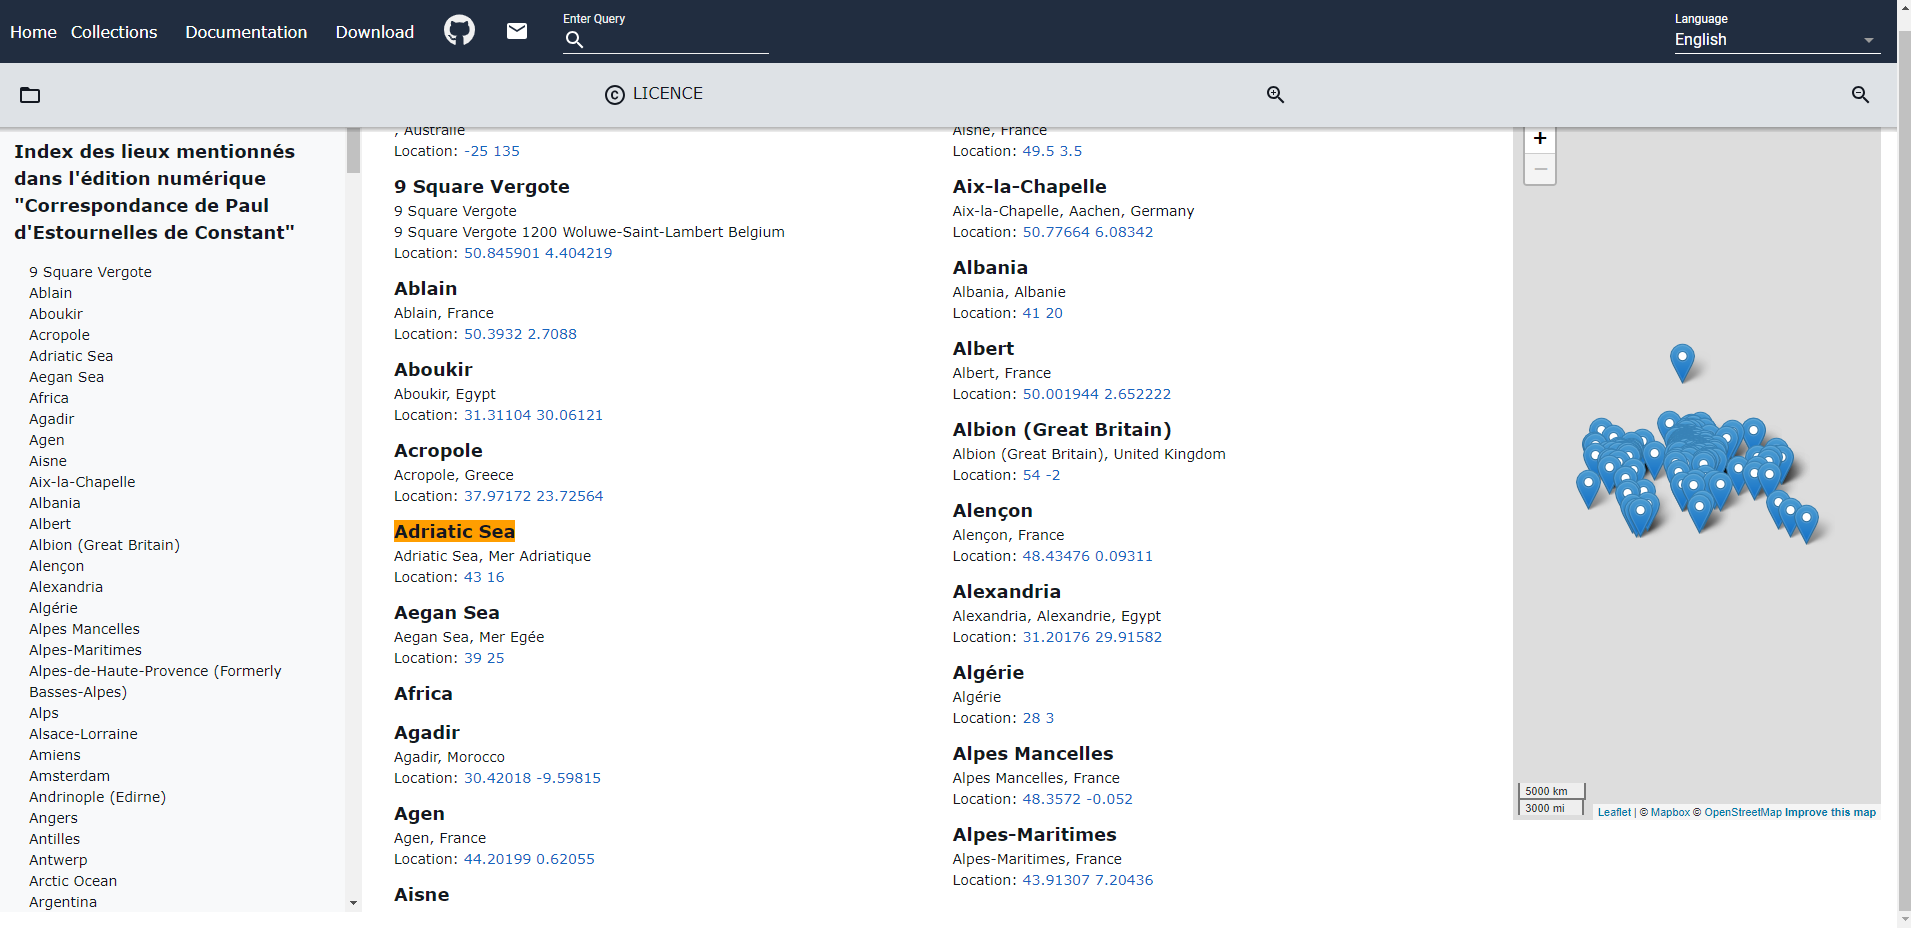
\includegraphics[width=1\linewidth]{schémas/index_places_old.png}
        \caption{Ancien index de DiScholEd}
        \label{fig:schémas18}
    \end{figure}
\begin{figure}[H]
        \centering
        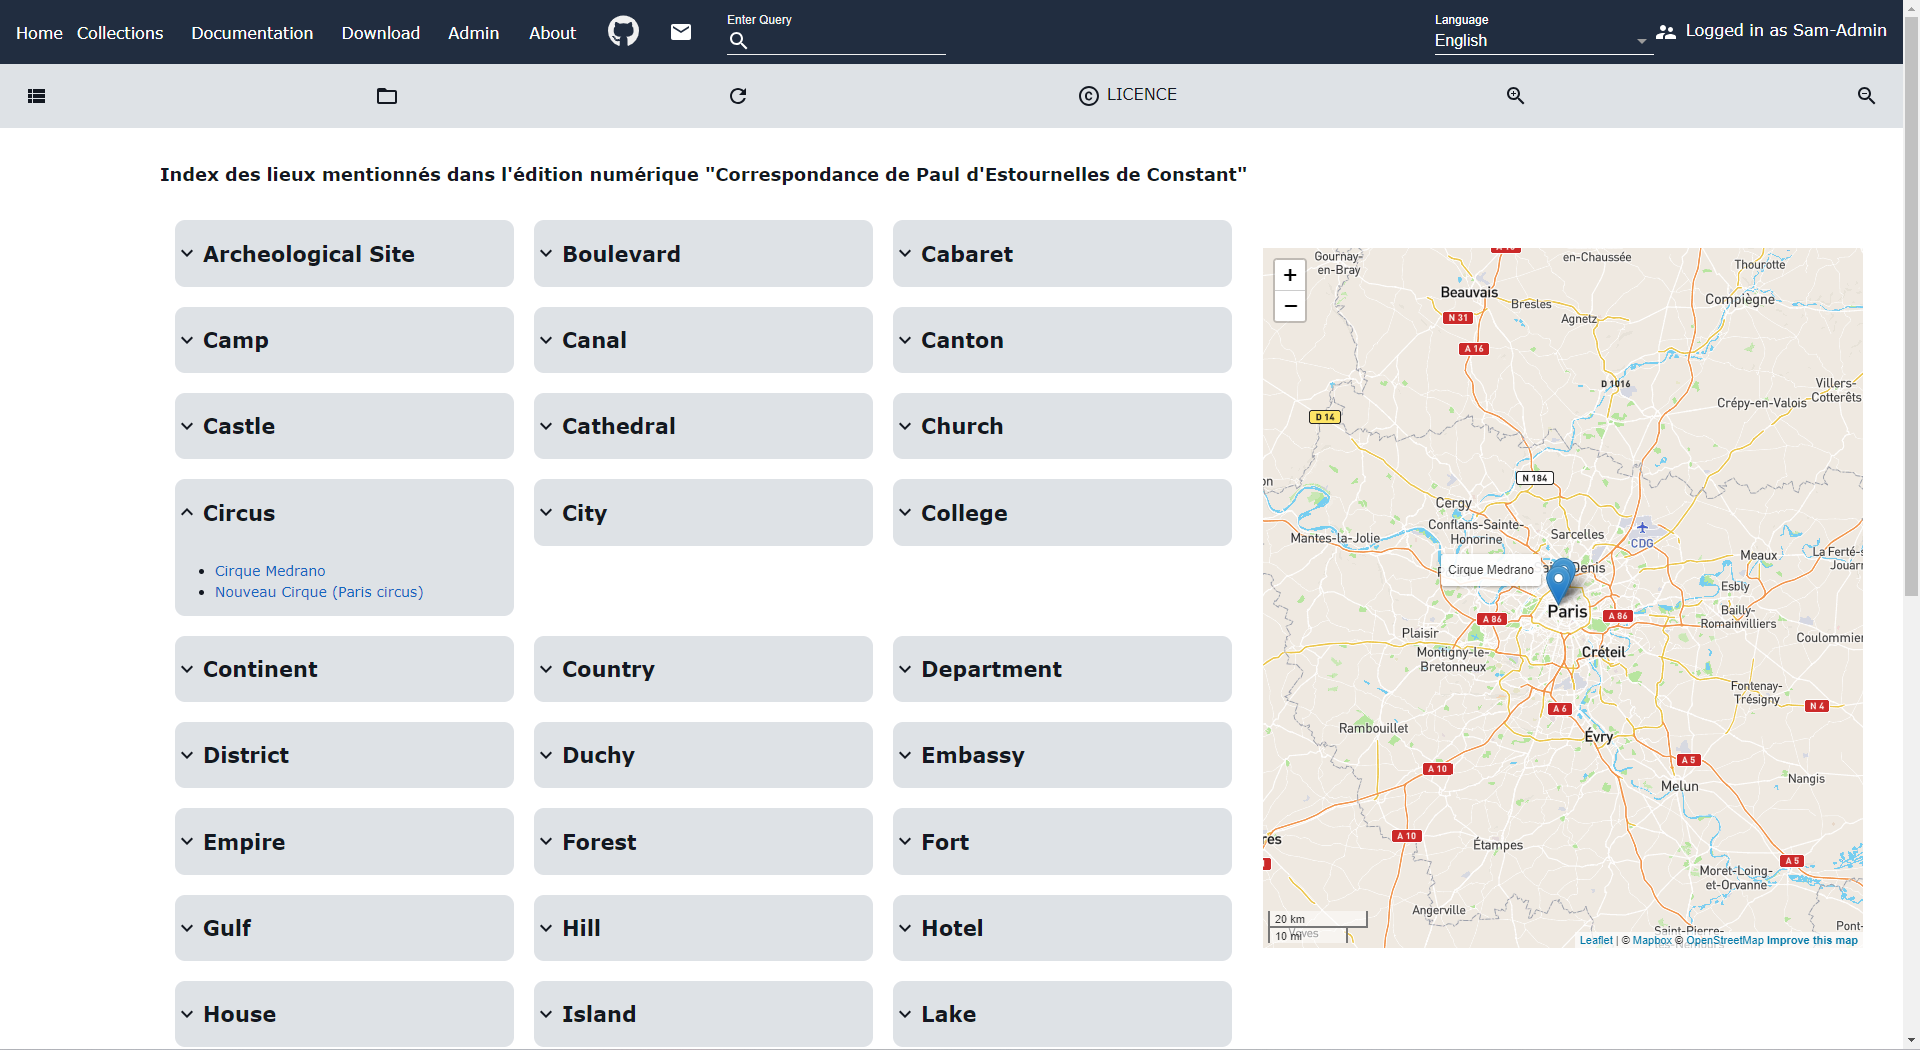
\includegraphics[width=1\linewidth]{schémas/index_places_new.png}
        \caption{Nouvel index de DiScholEd}
        \label{fig:schémas19}
    \end{figure}

\newpage

\section{Modifications des blocs de métadonnées pour toutes les langues}

\begin{figure}[H]
\centering
\begin{minipage}{.5\textwidth}
  \centering
  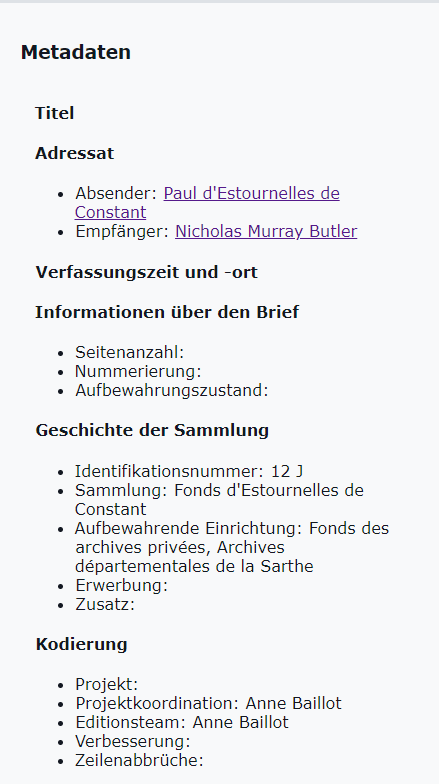
\includegraphics[width=.7\linewidth]{schémas/old_meta_deu.png}
  \caption{Ancien bloc de métadonnées}
  \label{old-meta-deu}
\end{minipage}%
\begin{minipage}{.5\textwidth}
  \centering
  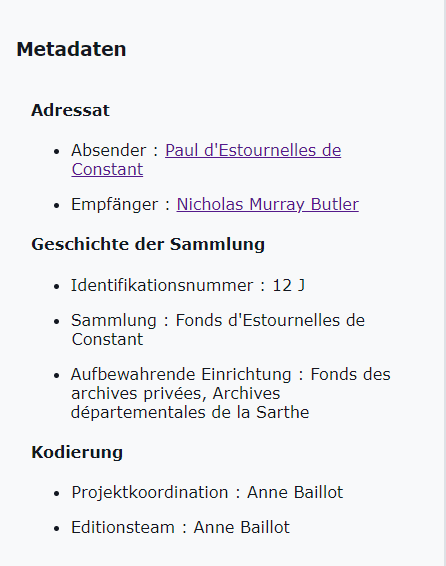
\includegraphics[width=.7\linewidth]{schémas/new-meta-deu.png}
  \caption{Nouveaux blocs de métadonnées sans les entrées où il n'y a pas d'information}
  \label{new-meta-deu}
\end{minipage}
\end{figure}

\newpage

\section{Amélioration de la page de présentation des collections}
\label{old_collection}
\begin{figure}[H]
        \centering
        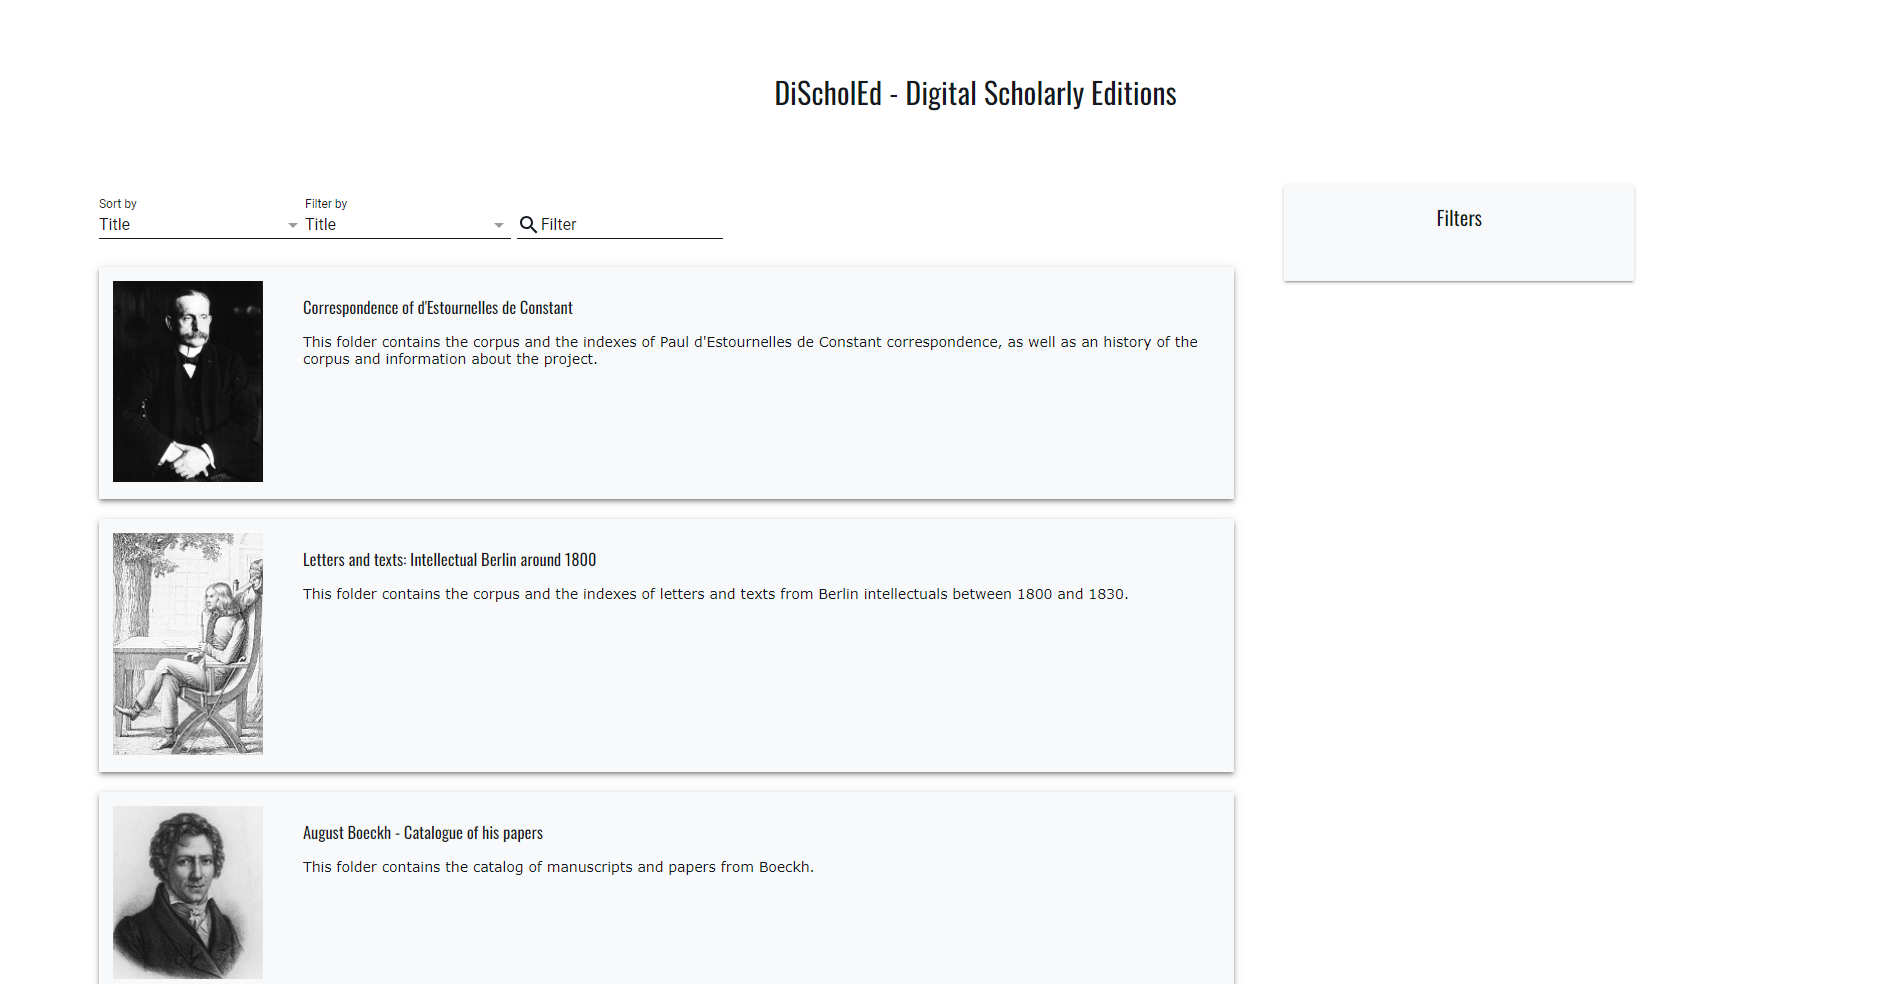
\includegraphics[width=1\linewidth]{schémas/old_collection.png}
        \caption{Ancienne page des collections}
        \label{fig:schémas22}
    \end{figure}
\label{new_collection}
\begin{figure}[H]
        \centering
        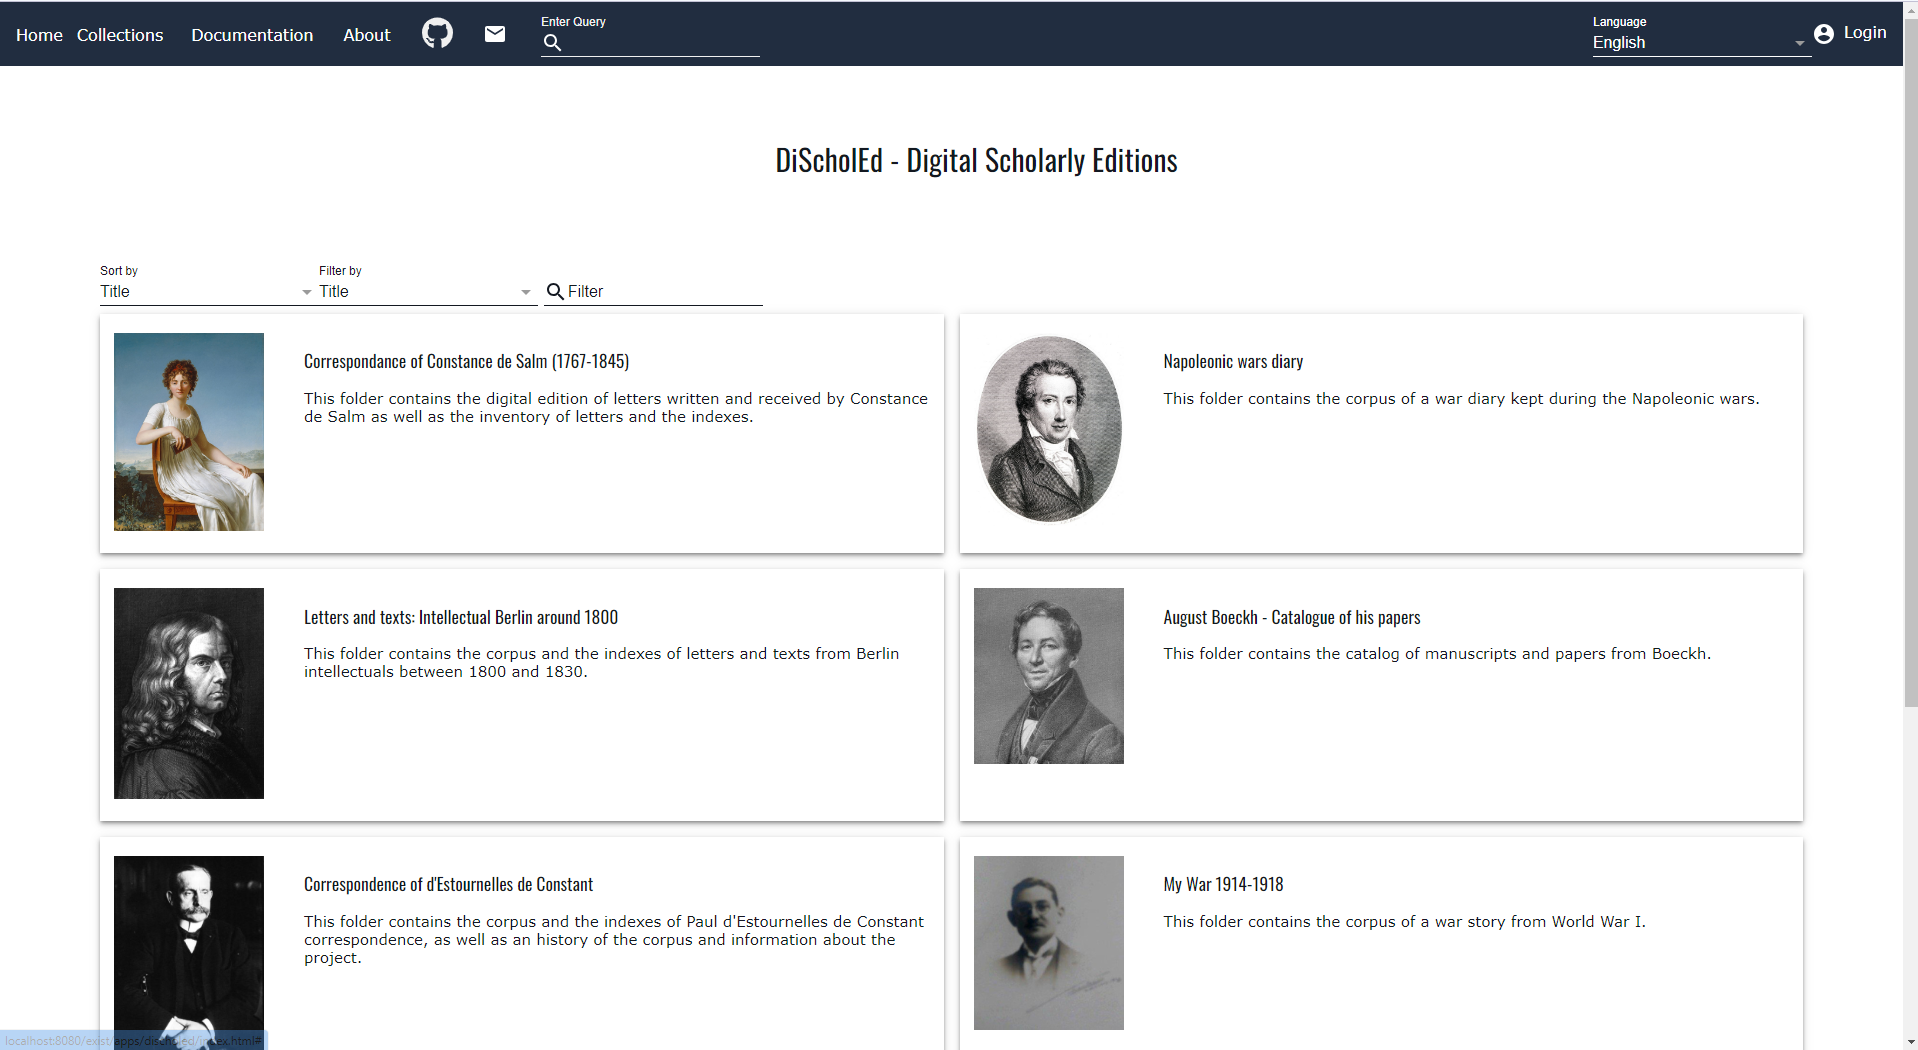
\includegraphics[width=1\linewidth]{schémas/new_collection.png}
        \caption{Nouvelle page des collections (meilleure qualité d'image, blocs cliquables, ordonnée par ordre alphabétique et en colonnes)}
        \label{fig:schémas23}
    \end{figure}

\newpage

\section{Suppression des langues indisponibles}

\begin{figure}[H]
\centering
\begin{minipage}{.5\textwidth}
  \centering
  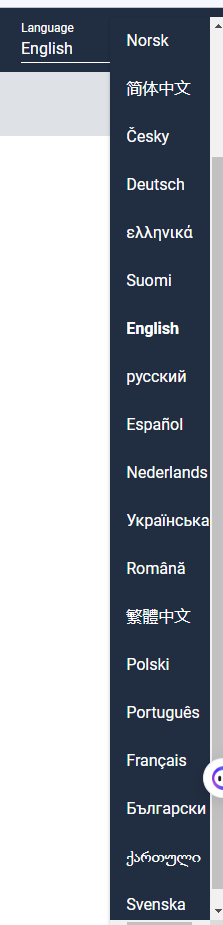
\includegraphics[width=.4\linewidth]{schémas/blangue.png}
  \caption{Anciennes langues non disponibles}
  \label{blangue}
\end{minipage}%
\begin{minipage}{.5\textwidth}
  \centering
  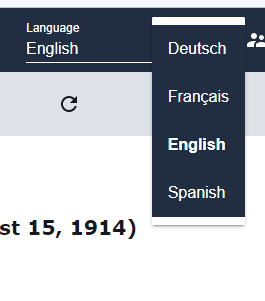
\includegraphics[width=.7\linewidth]{schémas/langue.png}
  \caption{Langues indisponibles de DiScholEd}
  \label{langue}
\end{minipage}
\end{figure}

    
    
%index à mettre ici si index	
%\printindex

% glossaire si glossaire
\printglossaries

% List of figures
\listoffigures
\addcontentsline{toc}{chapter}{Table des figures}

% Table of contents
\tableofcontents
\addcontentsline{toc}{chapter}{Table des matières}
	
\end{document}